\documentclass[xcolor={dvipsnames}]{beamer}
\usepackage{color, colortbl}
\usepackage[ngerman,english]{babel}
\usepackage[T1]{fontenc}
%\usepackage{CJKutf8} %japanese
\usepackage{lmodern}
%\usepackage{subfigure}
\usepackage[compatibility=false]{caption}
\usepackage{subcaption}
\usepackage{tikz}
\usetikzlibrary{calc}
\usepackage{textgreek}
\usepackage{array}
\usepackage{ragged2e}
\usepackage{tabularx}
\usepackage{booktabs}
\usepackage{xspace,multicol}
\usepackage{siunitx}
\usepackage{units}
\usepackage{appendixnumberbeamer}
\usepackage[absolute,overlay]{textpos} %for positioning the logos where I want

\usepackage{animate}
\usepackage{multimedia}
\usepackage{fixltx2e}
\usepackage{multicol}
\usepackage{comment}
\DeclareSIUnit\year{yr}
\newcommand{\lumi}{$\mathcal{L}$\xspace}

\mode<presentation>
{
  \usetheme{CambridgeUS}     
  \usecolortheme{lily} 
  \definecolor{beamer@violet}{rgb}{0.5,0.3,0.5} % changed this
  \setbeamercolor{structure}{fg=beamer@violet!70!cyan}
  \setbeamercolor{palette primary}{fg=black, bg=gray!30!white!50!cyan!20!}
  \setbeamercolor{palette secondary}{fg=black, bg=gray!30!white!30!cyan!40!}
  \setbeamercolor*{palette tertiary}{bg=gray!20!white!20!cyan!60!}
  
  \setbeamercolor{frametitle}{fg=cyan!60!white!40!,bg=cyan!80!black}
  \setbeamercolor{title}{fg=cyan!80!black}
  \setbeamercolor{normal text}{fg=black,bg=white}
  \setbeamercolor{alerted text}{fg=beamer@violet}
  \setbeamercolor{example text}{fg=beamer@violet!70!cyan}
  
  \usefonttheme{structureitalicserif} 
  \setbeamertemplate{navigation symbols}{}
  \setbeamertemplate{caption}[numbered]
}
\newcommand{\sidlogo}{
  \setlength{\TPHorizModule}{1pt}
  \setlength{\TPVertModule}{1pt}
   % textblock{}{x,y}: pos(x) = rightUpperCorner + (x * \TPHorizModule), pos(y) = leftUpperCorner - (y * \TPVertModule)
  \begin{textblock}{1}(323,12)
   
\includegraphics[width=40pt,height=26pt]{figures/SiD.jpeg}
  \end{textblock}
  } 
\newcommand{\ilclogo}{
  \setlength{\TPHorizModule}{1pt}
  \setlength{\TPVertModule}{1pt}
   % textblock{}{x,y}: pos(x) = rightUpperCorner + (x * \TPHorizModule), pos(y) = leftUpperCorner - (y * \TPVertModule)
  \begin{textblock}{1}(323,12)
   
\includegraphics[width=40pt,height=26pt]{figures/ILC.jpeg}
  \end{textblock}
} 
\newcommand{\ejadelogo}{
  \setlength{\TPHorizModule}{1pt}
  \setlength{\TPVertModule}{1pt}
   % textblock{}{x,y}: pos(x) = rightUpperCorner + (x * \TPHorizModule), pos(y) = leftUpperCorner - (y * \TPVertModule)
  \begin{textblock}{1}(323,12)
   
\includegraphics[width=40pt,height=26pt]{figures/EJADE.jpeg}
  \end{textblock}
} 
\newcommand{\ATFlogo}{
  \setlength{\TPHorizModule}{1pt}
  \setlength{\TPVertModule}{1pt}
   % textblock{}{x,y}: pos(x) = rightUpperCorner + (x * \TPHorizModule), pos(y) = leftUpperCorner - (y * \TPVertModule)
  \begin{textblock}{1}(323,12)
   
\includegraphics[width=40pt,height=26pt]{figures/ATF_logo.jpg}
  \end{textblock}
} 
\newcommand{\RHULlogo}{
  \setlength{\TPHorizModule}{1pt}
  \setlength{\TPVertModule}{1pt}
   % textblock{}{x,y}: pos(x) = rightUpperCorner + (x * \TPHorizModule), pos(y) = leftUpperCorner - (y * \TPVertModule)
  \begin{textblock}{1}(337,12)
   
\includegraphics[width=25pt,height=26pt]{figures/rhul_logo.png}
  \end{textblock}
}
\newcommand{\flukalogo}{
  \setlength{\TPHorizModule}{1pt}
  \setlength{\TPVertModule}{1pt}
   % textblock{}{x,y}: pos(x) = rightUpperCorner + (x * \TPHorizModule), pos(y) = leftUpperCorner - (y * \TPVertModule)
  \begin{textblock}{1}(315,12)
   
\includegraphics[width=60pt,height=26pt]{figures/fluka_logo.png}
  \end{textblock}
} 

\newcommand{\electron}{e$^-$}
\newcommand{\positron}{e$^+$}

\title[ILC \& Background Simulations]{\textbf{\LARGE The International Linear Collider\\ \large -\\ Background Simulations \& \\Optimizations of the Final-Focus Region \\\vspace*{0.2cm} \small GK Workshop, Bad Liebenzell}}
\author{\textbf{Anne Sch\"utz}}
\institute{\textbf{KIT, DESY}}
\date{\textbf{11. October 2017}}

\titlegraphic{
\includegraphics[height=1.0cm]{figures/KIT.png}\hspace*{6cm}~%
   
\includegraphics[height=1.2cm]{figures/DESY_Logo.png}
}

\begin{document}

{
\usebackgroundtemplate{
 \tikz\node[opacity=0.1]{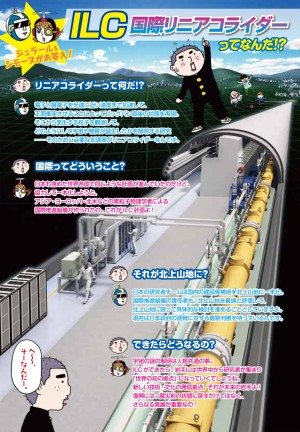
\includegraphics[width=\paperwidth]{figures/Iwatecomics.jpg}};
 % \tikz\node[opacity=0.2]{\centering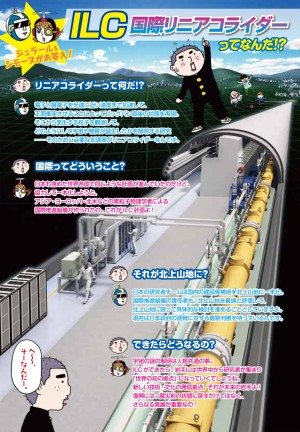
\includegraphics[height=\paperheight]{figures/Iwatecomics.jpg}};
 }
\begin{frame}
  \titlepage
\end{frame}
}

\begin{frame}{Table of contents}
\begin{multicols}{2}
  \tableofcontents
\end{multicols}
\end{frame}


\section{What would an ideal particle collider be like?}

\newcolumntype{R}[1]{>{\RaggedLeft\arraybackslash}p{#1}}
\newcolumntype{C}[1]{>{\centering}p{#1}}
\newcolumntype{L}[1]{>{\RaggedRight\arraybackslash}p{#1}}
%\newcolumntype{L}[1]{>{\raggedright\let\newline\\\arraybackslash}p{#1}}

\begin{frame}
 \begin{center}
  {\LARGE If YOU could build a particle collider,\\what would it be like?}
 \end{center}
  \vspace*{0.2cm}
\alert{\large
\begin{table}
\centering
\begin{tabular}{R{5.5cm} C{0.2cm} L{6cm}}
\visible<2->{Highest energies} & \visible<4->{$\rightarrow$} & \visible<4->{Circular hadron collider} \\
\visible<2->{Highest precision} & \visible<4->{$\rightarrow$} & \visible<4->{Lepton collider} \\
\visible<2->{``No'' background} & \visible<4->{$\rightarrow$} & \visible<4->{Lepton collider}\\
\visible<2->{Several experiments (detectors)} & \visible<4->{$\rightarrow$} & \visible<4->{\textit{Usually} only collider rings}\\
\visible<2->{Cheap} & \visible<5->{$\rightarrow$} & \visible<5->{\textbf{ILC}}\\
\visible<3->{Feasible to be built before we are pensioners!} & \visible<5->{$\rightarrow$} & \visible<5->{\textbf{ILC}}
\end{tabular}
\end{table}
}
\end{frame}
%--------------------------------------------------------------
\subsection{Physics motivation of a lepton collider}
\begin{frame}[fragile]{The physics motivation of a lepton collider}
\ilclogo

\begin{block}{}
\centering
\textcolor{JungleGreen}{Cleanliness} - \textcolor{WildStrawberry}{Democracy} - \textcolor{Periwinkle}{Calculability} - \textcolor{LimeGreen}{Detail}
\end{block}

\visible<2->{
\begin{overprint}
\onslide<2>
\begin{itemize}
\color{JungleGreen}
\item Small background
\item Due to polarization, background can be ``switched off''
\item Small detector occupancy
\item Smaller energy range
\item No out-of-time pileup or underlying events
\end{itemize}
\centering
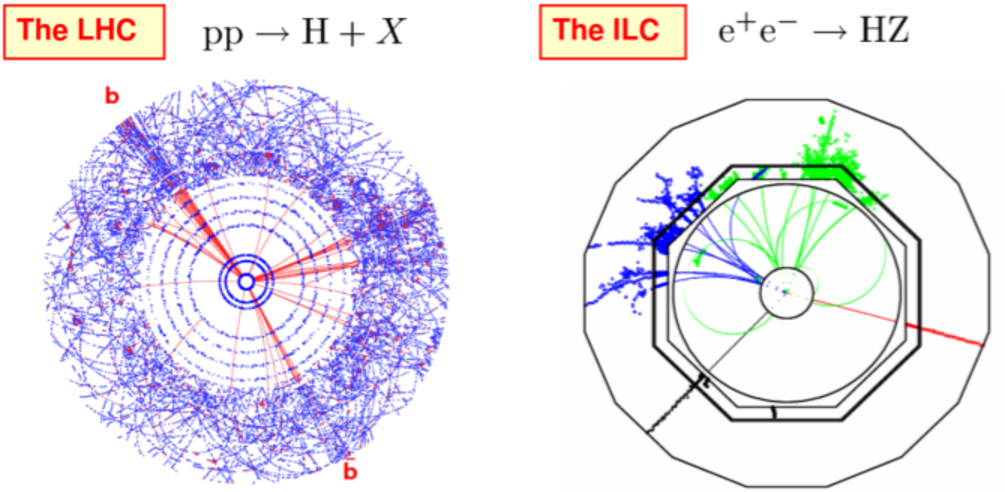
\includegraphics[width=0.6\textwidth]{figures/ILC_LHC_eventdisplay_comparison.pdf}

\onslide<3>
\begin{itemize}
\color{WildStrawberry}
\item Elementary coupling \textit{e} of photons is the same for all quarks and leptons
\item e$^+$e$^-$ annihilation produces pairs of all species, SM and exotics, at similar rates
\item Model independence
\item No triggers
\end{itemize}

\onslide<4>
\begin{itemize}
\color{Periwinkle}
\item Point-like elementary particles in initial state
\item Coupling only to electroweak interactions
\item No systematic uncertainties due to PDF uncertainties and QCD corrections
\end{itemize}

\onslide<5>
\begin{itemize}
\color{LimeGreen}
\item Reconstruction of complete events
\item Quark and lepton momenta determined by kinematic fits
\item Due to high energy resolution, particles with small mass difference distinguishable $\rightarrow$ Peaks are measurable that weren't measurable before
\item c-tagging possible because of small distance between IP and the detector (nano-sized beam !)
\end{itemize}

\onslide<6>
\begin{columns}
\begin{column}{0.24\textwidth}
\begin{itemize}
\color{JungleGreen}
\item Small background
\item Small detector occupancy
\item Smaller energy range
\item No out-of-time pileup or underlying events
\end{itemize}
\end{column}
\begin{column}{0.26\textwidth}
\begin{itemize}
\color{WildStrawberry}
\item Elementary coupling \textit{e} of \textgamma \, the same for all quarks \& leptons
\item e$^+$e$^-$ annihilation produces pairs of all species, SM \& exotics, at similar rates
\item No triggers
\end{itemize}
\end{column}
\begin{column}{0.27\textwidth}
\begin{itemize}
\color{Periwinkle}
\item Pointlike elementary particles in initial state
\item Coupling only to EW interactions
\item No sys. uncert. due to PDF uncertainties and QCD corrections
\end{itemize}
\end{column}
\begin{column}{0.27\textwidth}
\begin{itemize}
\color{LimeGreen}
\item Reconstruction of complete events
\item Quark \& lepton momenta determined by kinematic fits
\item High energy resolution
\item c-tagging
\end{itemize}
\end{column}
\end{columns}
\end{overprint}
}%end visible
\end{frame}

\section{The International Linear Collider}

\subsection{The layout}
\begin{frame}{The layout of the ILC}
\ilclogo

e$^+$e$^-$ linear collider with adjustable center-of-mass energy, and polarized beams\\
\begin{center}
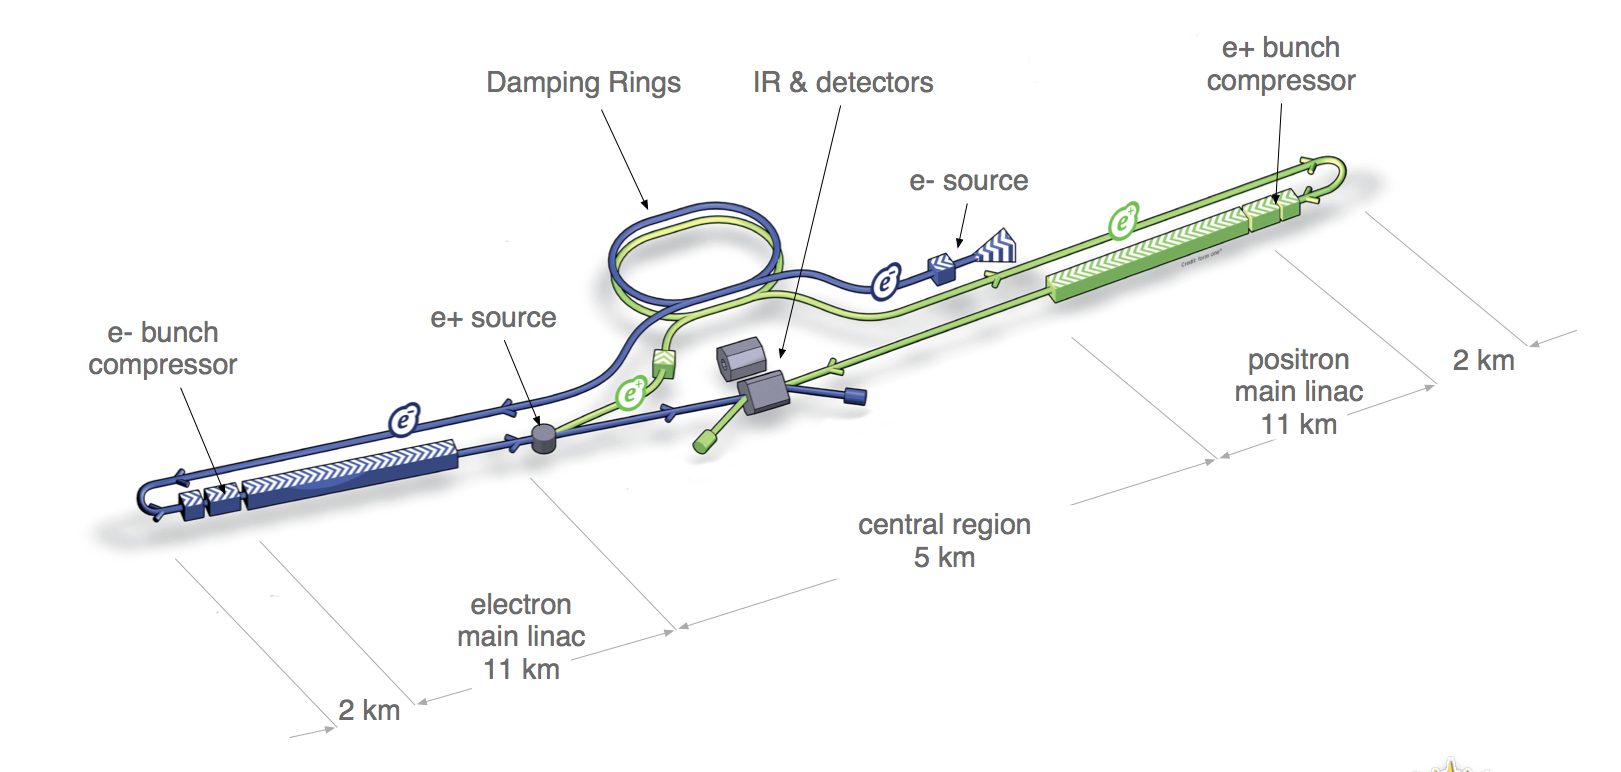
\includegraphics[width=\textwidth]{figures/ILC_schematic_layout.png}
\end{center}
\end{frame}

\begin{frame}{Why linear?}
\begin{columns}
 \begin{column}{0.6\textwidth}
  Basic limitations of lepton synchrotons:
\begin{itemize}
 \item \textcolor{Red}{Energy loss due to synchrotron radiation: $\sim$ E$^4$/R}
 \item \textcolor{Red}{Cost $\sim$ quadratically with energy}\\ \tiny{(B. Richter 
1980)}
\end{itemize}
\vspace*{1cm}
Therefore a linear collider:
\begin{itemize}
 \item \textcolor{ForestGreen}{Not limited by synchrotron radiation}
 \item \textcolor{ForestGreen}{Cost $\sim$ linear with energy}
\end{itemize}
 \end{column}
 \begin{column}{0.4\textwidth}
 \begin{block}{}
  \begin{center}
      \textcolor{Gray}{P$_S=\frac{e^2c}{6\pi\epsilon_0}\frac{1}{(m_0c^2)^4}\frac{E^4}{R^2}$\\
  $\Delta$E$=\frac{e}{3\epsilon_0(m_0c^2)^4}\frac{E^4}{R}$}
   \end{center}
 \end{block}
 \end{column}
\end{columns}

\end{frame}

\AtBeginSubsection[]
{
  \begin{frame}<beamer>
     \tableofcontents[currentsection,
     currentsubsection,
     %hideothersubsections,
     subsectionstyle=show/shaded/hide,
     subsubsectionstyle=show/show/hide]
  \end{frame}
}

\subsection{The candidate site of the ILC}
\begin{frame}{The candidate site - The Kitakami mountains}
\ilclogo
\begin{center}
\begin{minipage}[t]{0.49\textwidth}
\centering
 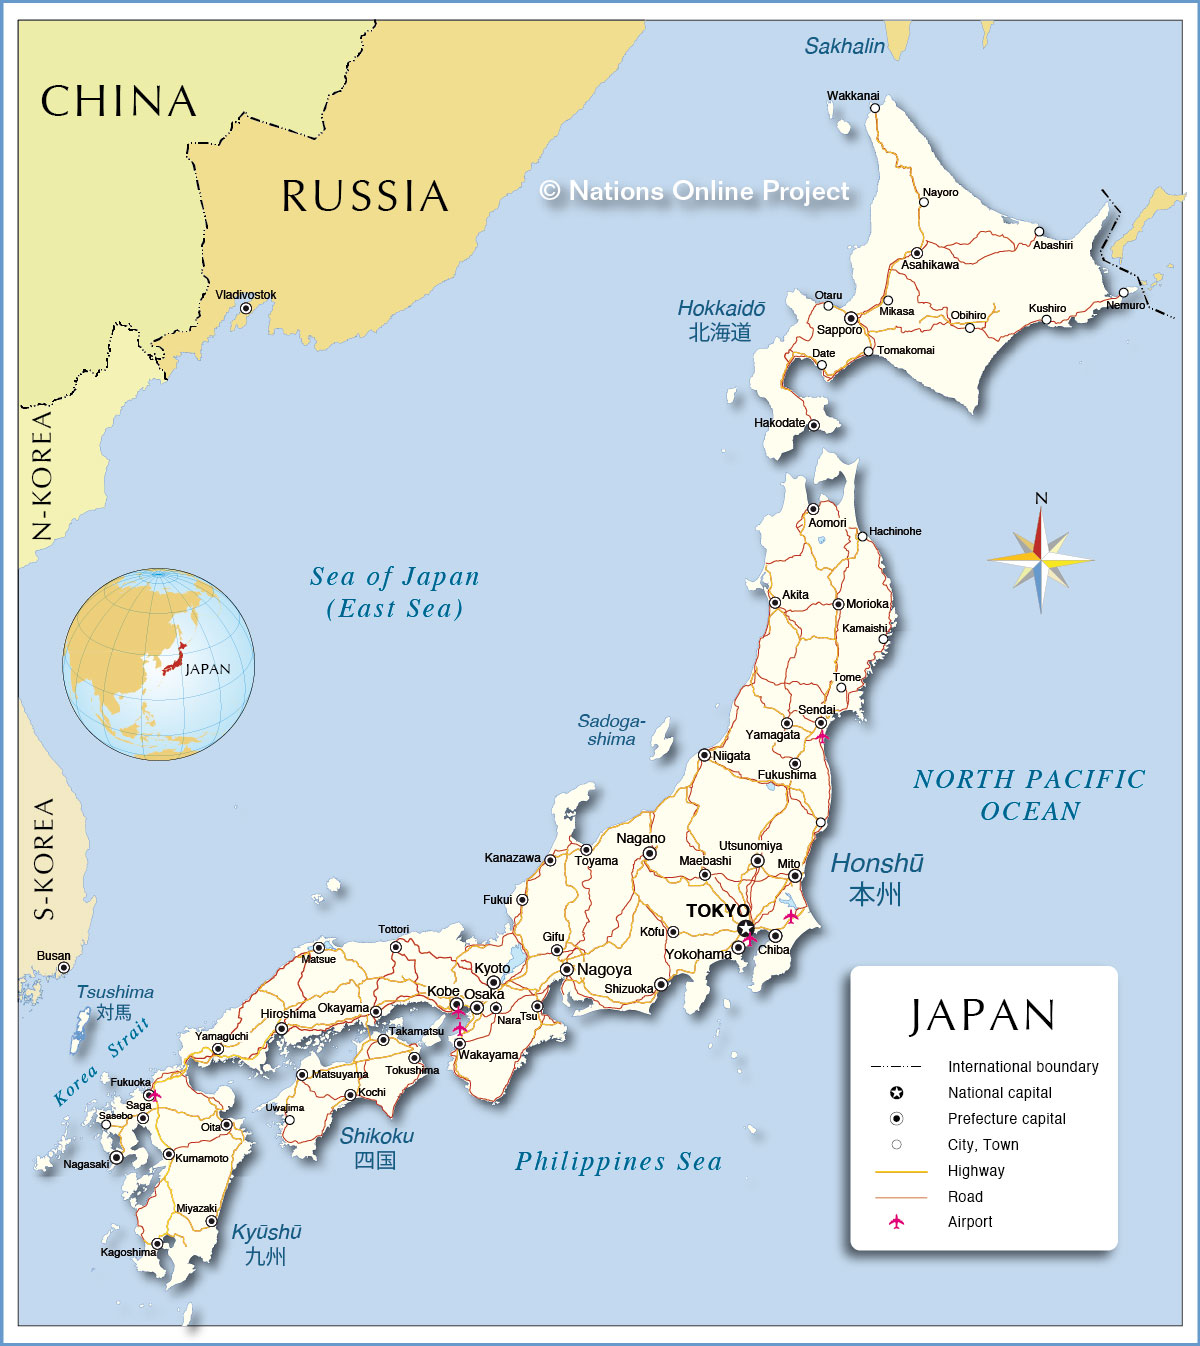
\includegraphics[width=\textwidth]{figures/japan-map.jpg}
\end{minipage}
\begin{minipage}[t]{0.48\textwidth}
\centering
   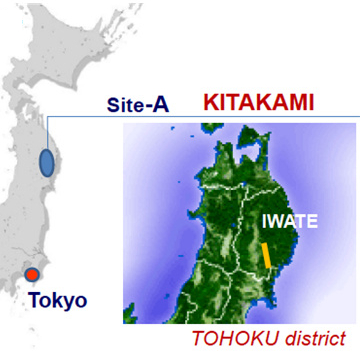
\includegraphics[width=\textwidth]{figures/Kitakami_site.jpg}
\end{minipage}
\end{center}
\end{frame}



%------Definition for column color in table
\definecolor{Gray}{gray}{0.9}
\newcolumntype{g}{>{\columncolor{Gray}}r}
%-----------------------------------------
\subsection{The beam parameters}
\begin{frame}{The beam parameters of the \textbf{ILC}}
\ilclogo
\begin{center}
\begin{tikzpicture}
\node (table) {\input{table_ILCparameters.tex}};
\visible<3>{\draw [red,ultra thick,rounded corners]
  ($(table.south west) !.46! (table.north west)$)
  rectangle 
  ($(table.south east) !.64! (table.north east)$);}
\visible<4>{\draw [red,ultra thick,rounded corners]
  ($(table.south west) !.19! (table.north west)$)
  rectangle 
  ($(table.south east) !.37! (table.north east)$);}
\visible<2>{\draw [red,ultra thick,rounded corners]
  ($(table.south west) !.01! (table.north west)$)
  rectangle 
  ($(table.south east) !.12! (table.north east)$);}
\end{tikzpicture}
\end{center}
\end{frame}

\subsection{The detectors}
\begin{frame}{The two detectors - SiD and ILD}
\ilclogo
\begin{block}{}
The ILC has only one Interaction Point (IP).\\
The two detectors can be swapped in the so-called \textbf{push-pull-system}.
\end{block}

\begin{columns}
\begin{column}{0.48\textwidth}
\begin{center}
\alert{SiD - Silicon Detector}
\begin{itemize}
\item Height: $\sim$\SI{14}{\metre}, length:  $\sim$\SI{11}{\metre}
\item Weight: $\sim$\SI{10100}{\tonne}
\item Superconducting solenoid field: \SI{5}{\tesla}
\item Full silicon tracker
\end{itemize}

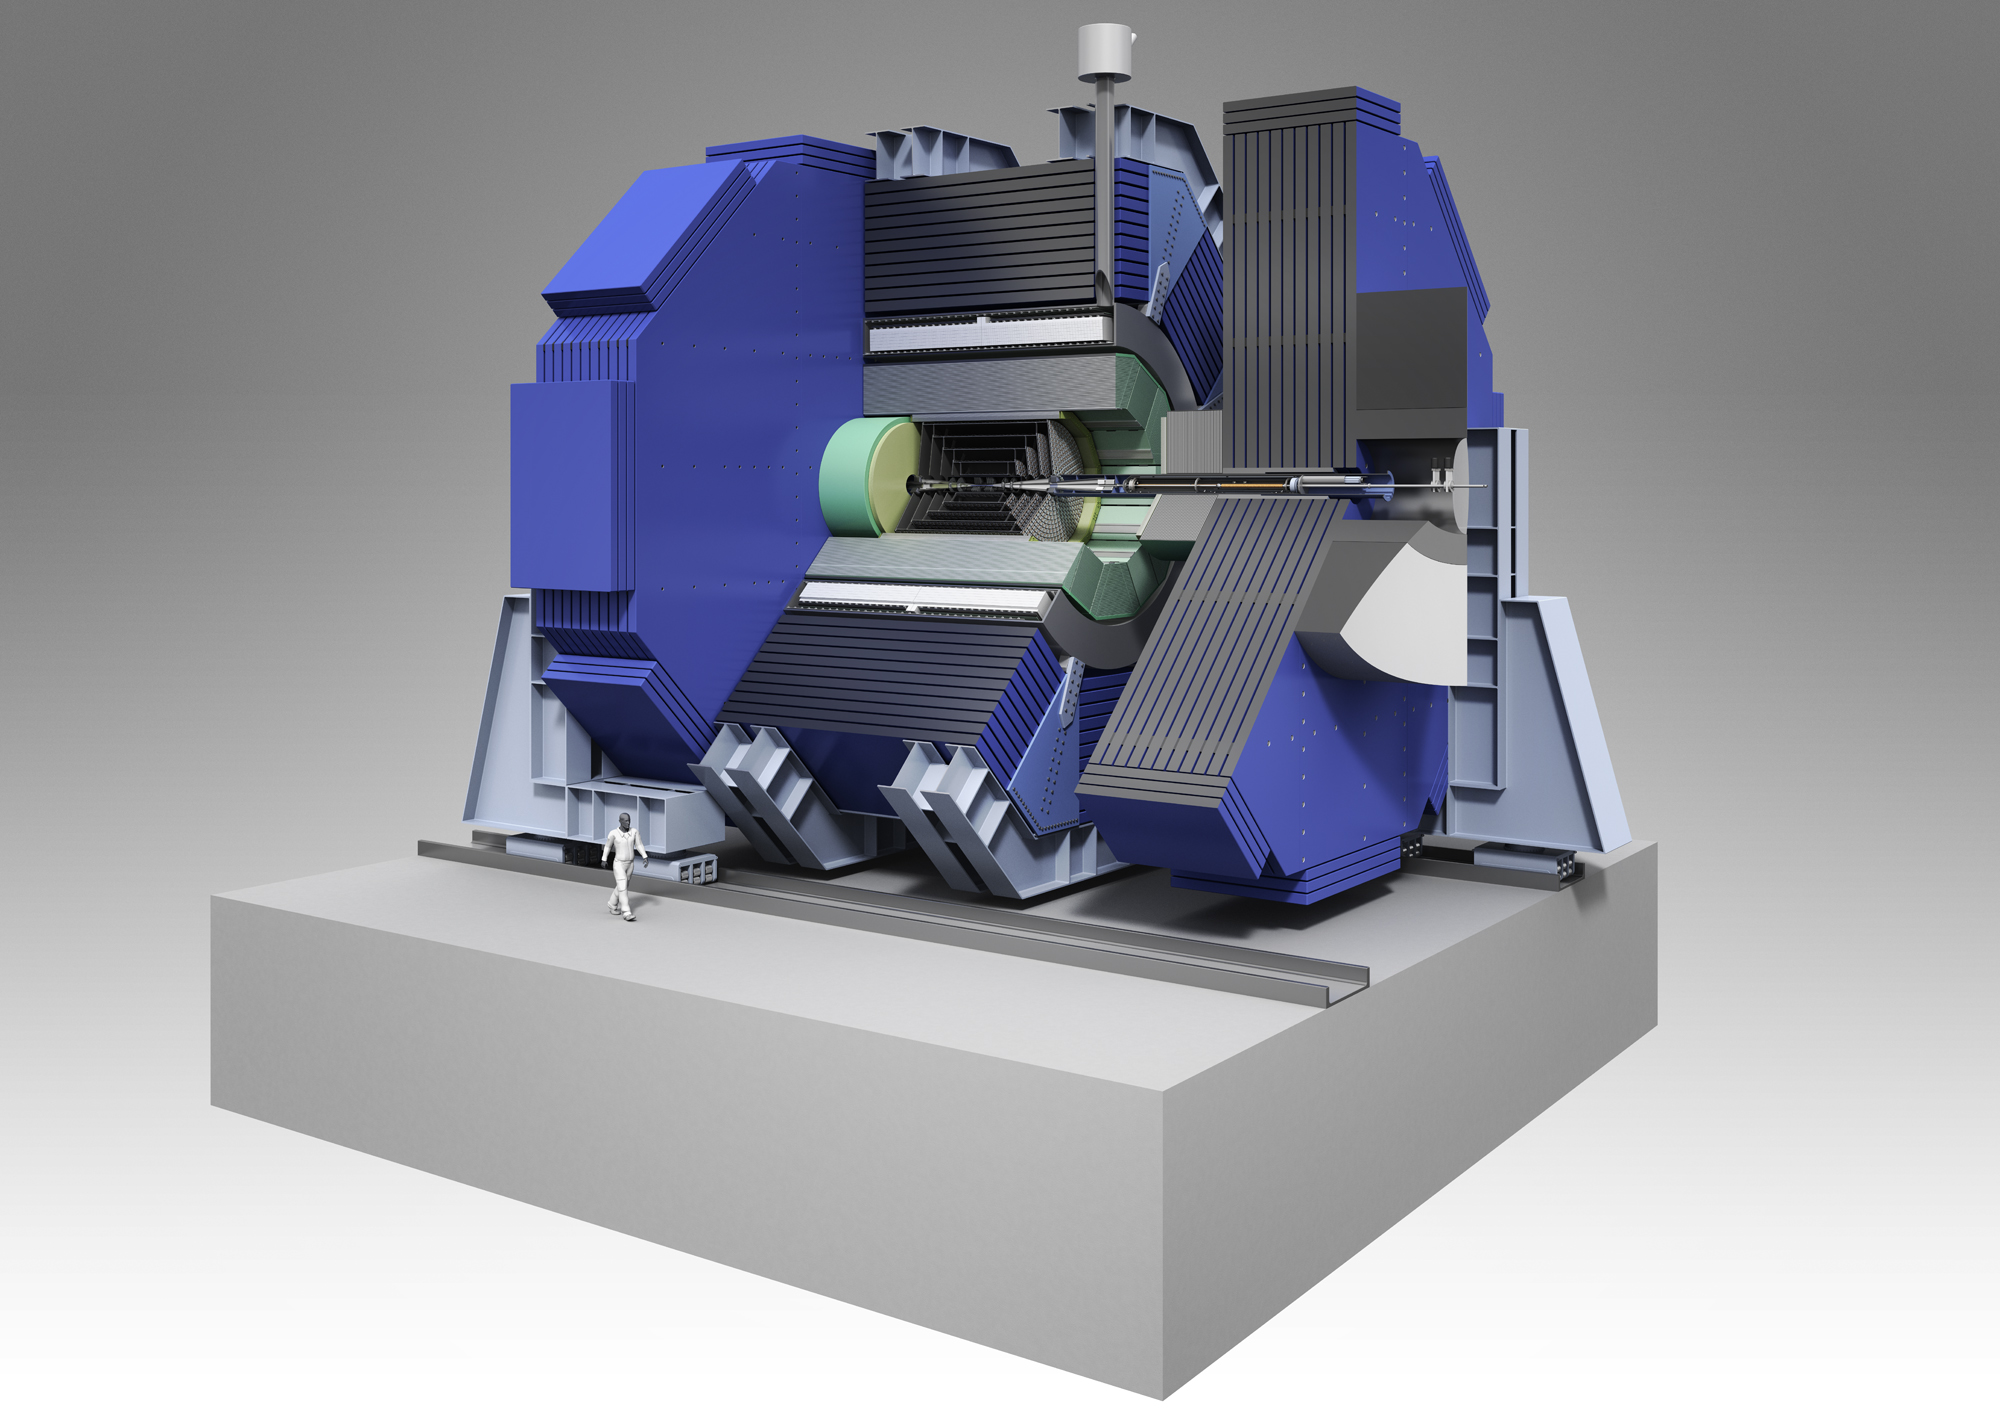
\includegraphics[width=0.5\textwidth]{figures/SiDmodel.jpg}

\end{center}
\end{column}

\begin{column}{0.48\textwidth}
\begin{center}
\alert{ILD - International Large Detector}
\begin{itemize}
\item Height: $\sim$\SI{16}{\metre}, length:  $\sim$\SI{14}{\metre}
\item Weight: $\sim$\SI{14000}{\tonne}
\item Superconducting solenoid field: \SI{3.5}{\tesla}
\item TPC
\end{itemize}

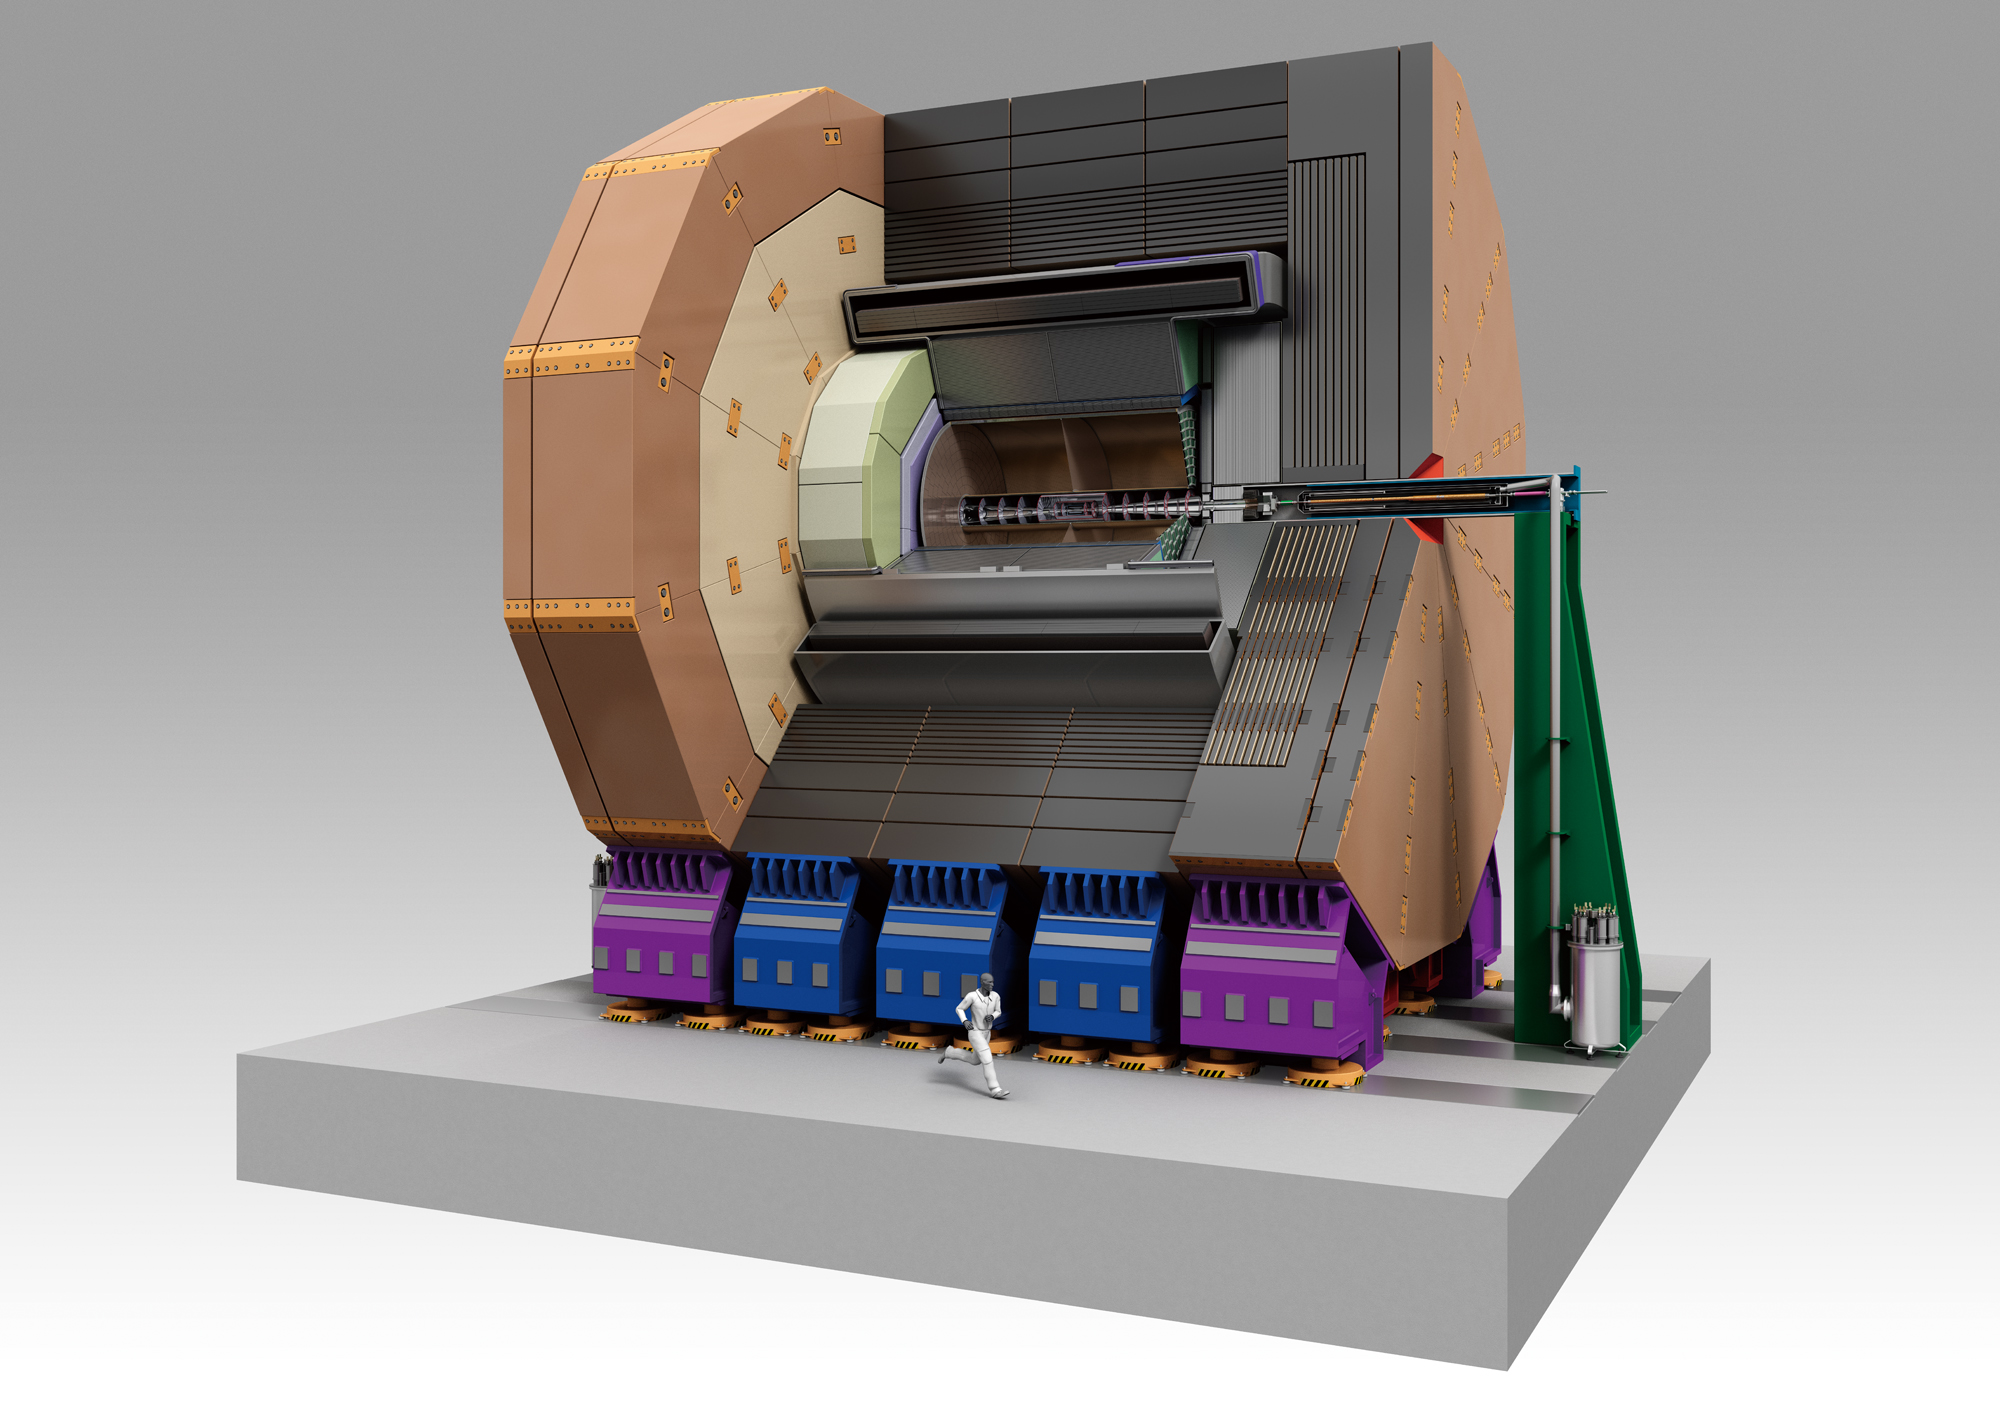
\includegraphics[width=0.5\textwidth]{figures/ILDmodel.jpg}

\end{center}
\end{column}
\end{columns}
\end{frame}

\subsubsection{SiD detector}
\begin{frame}{SiD detector}
\sidlogo
 I am in the SiD-Optimization group.\\
 Marcel Stanitzki is currently the SiD co-spokesperson.\\
 \vspace*{0.3cm}
 \begin{columns}
  \begin{column}{0.7\textwidth}
    SiD has a very convincing design:
 \begin{itemize}
  \item compact and robust
  \item full silicon vertex detector and tracker
  \\Vertex detector:
  \begin{itemize}
   \item $<$\SI{5}{\micro\metre} resolution
   \item Momentum resolution $\sim$ 2-\SI{5e-5}{\per\giga\electronvolt}
   \item $\sim$ \SI{0.1}{\percent} X$_0$ per layer
  % \item Single bunch timing resolution
  % \item cos($\theta$)$\approx$0.984
  \end{itemize}

  \item highly granular calorimetry optimized for Particle Flow (ECAL: radation length = 26 X$_0$, \\EM energy resolution = 0.17/$\sqrt{E}\bigoplus$1\%)
 \end{itemize}
  \end{column}
  \begin{column}{0.3\textwidth}
    \begin{flushright}
  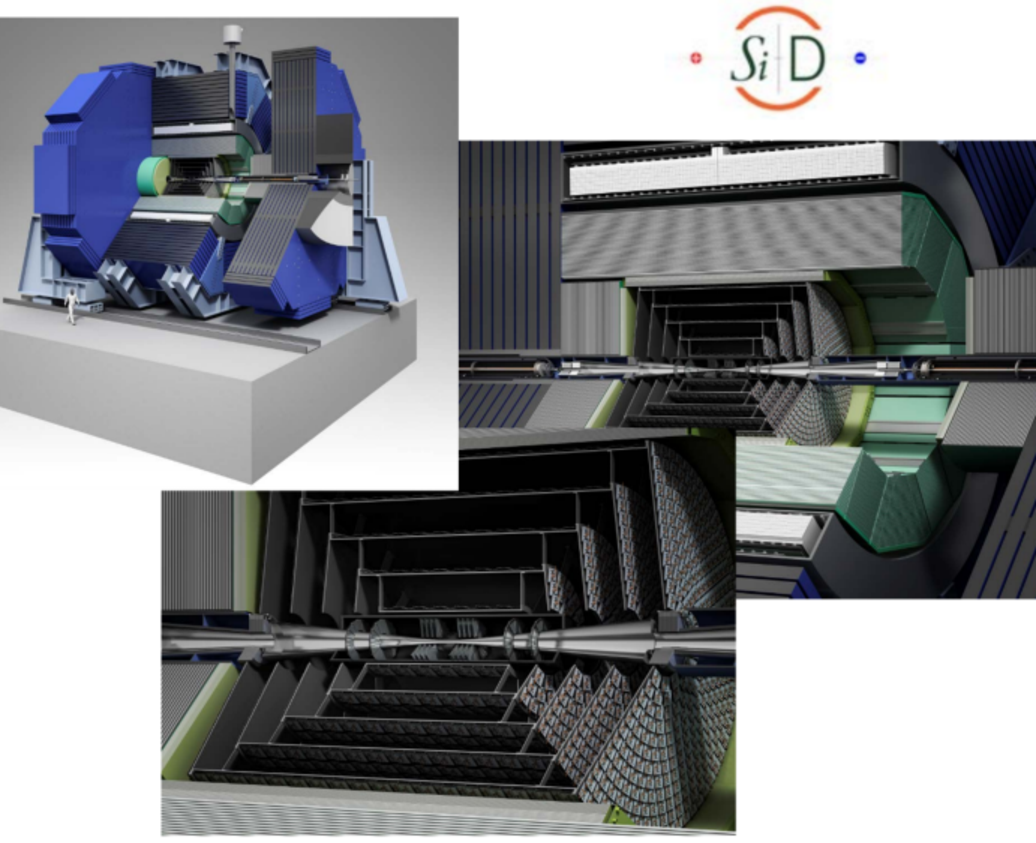
\includegraphics[height=0.4\textheight]{figures/SiDpics.pdf}
 \end{flushright}
  \end{column}
 \end{columns}
\end{frame}

\begin{frame}{SiD detector}
\sidlogo
\begin{figure}[T]
\centering
\begin{subfigure}[b]{0.49\textwidth}
\centering
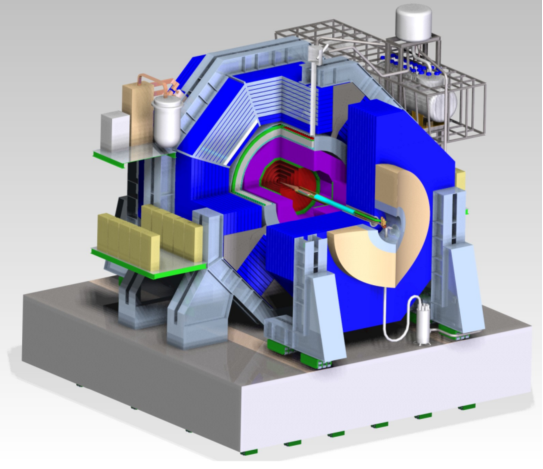
\includegraphics[height=0.65\textheight]{figures/SiD_detector_model.pdf}
\end{subfigure}
\begin{subfigure}[b]{0.49\textwidth}
\centering
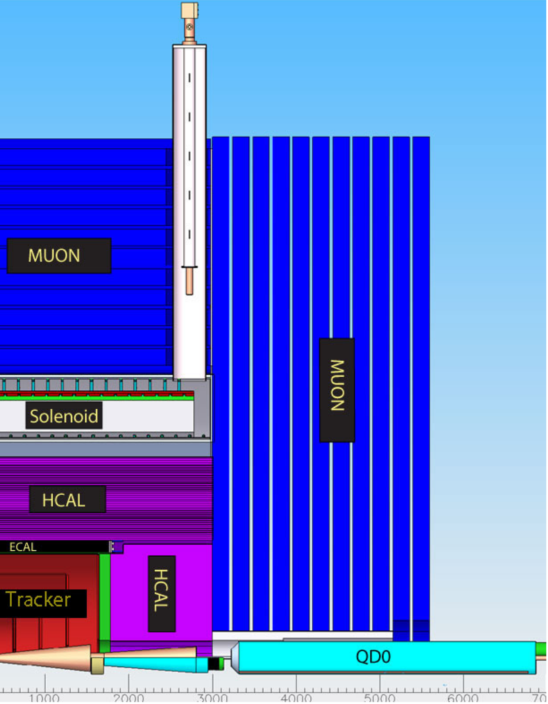
\includegraphics[height=0.65\textheight]{figures/SiD_detector_model_Ausschnitt.pdf}
\end{subfigure}
\end{figure}
{\small SiD detector model: Vertex detector (red), ECAL (green), HCAL (pink), Muon system (blue)}
\end{frame}


\subsection{Physics Goals}
\begin{frame}{Physics goals for the different ILC stages}
\begin{center}
  \includegraphics[width=0.7\textwidth]{figures/Physics_Goals.png}
\end{center}
We want to do PRECISION measurements, and find new particles and new physics! :)
\end{frame}
\begin{frame}{Higgs coupling precisions}
\ilclogo
ILC: Each Higgs coupling will be measured to a \alert{percent accuracy}, \alert{direct measurement of the global width} of the Higgs.\\
LHC: \alert{Global fit to all Higgs signals} (plus using \alert{theoretical assumptions} of the width) $\rightarrow$ Higgs couplings can never be as precise as at the ILC\\ \vspace*{0.3cm}
\centering \includegraphics[width=0.6\textwidth]{figures/PhysicsMotivation-Peskin_PrecisionHiggsCouplings.png}
\end{frame}

\AtBeginSection[]
{
  \begin{frame}<beamer>
     \tableofcontents[currentsection,
     currentsubsection,
     %hideothersubsections,
     subsectionstyle=show/shaded/hide,
     subsubsectionstyle=show/show/hide]
  \end{frame}
}

\section{Latest News from the ILC}
\begin{frame}{Down grading the ILC?}
 \alert{The Japanese government asks for a \textbf{significant} cost reduction.}\\ \vspace*{0.3cm}
 \visible<2->{
 To achieve such a dramatic cost reduction, the full machine needs to be staged.\\
 \alert{Instead of \SI{500}{GeV} center-of-mass energy} as the first stage, it was decided to start with \alert{\SI{250}{GeV}}.\\
 This comes with revisiting the machine parameters $\rightarrow$ increasing the possible luminosity $\rightarrow$ increasing the possible physics outcome.
 }
 \visible<3->{
 \vspace*{0.3cm}\\
 In order to increase the luminosity, the horizontal emittance $\epsilon_x$ is reduced.\\
 \textcolor{Red}{Downside:\\
 This leads to stronger beam-beam interactions, and therefore larger backgrounds!}\\
 Work in progress:\\
 Looking at effects on the SiD detector. Maybe the detector design has to be changed!
 }
\end{frame}


\section{Background simulations}
\subsection{Background sources}

\begin{frame}{Background sources}
\ilclogo
The main sources of background:
\begin{columns}
 \begin{column}{0.6\textwidth}
  \begin{itemize}
    \item Beam-beam interactions:
    \begin{itemize}
      \item \textbf{Pair background}
      \item Bhabha scattering
      \item \textgamma \textgamma $\rightarrow$ hadrons
    \end{itemize}
    \vspace*{0.5cm}
    \item Machine background:
    \begin{itemize}
      \item Muons from the Beam Delivery System
      \item Background from the Final-Focus system (beam halo collimators)
      \item \textbf{Neutrons from the Main Beam Dumps}
    \end{itemize}
  \end{itemize}
 \end{column}
 \begin{column}{0.45\textwidth}
 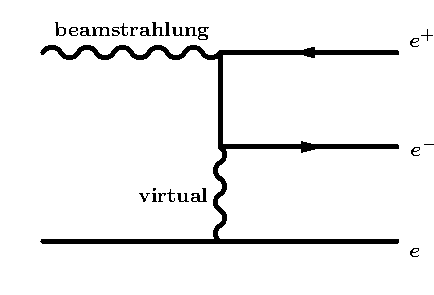
\includegraphics[width=0.48\textwidth]{figures/Bethe-Heitler.pdf}
 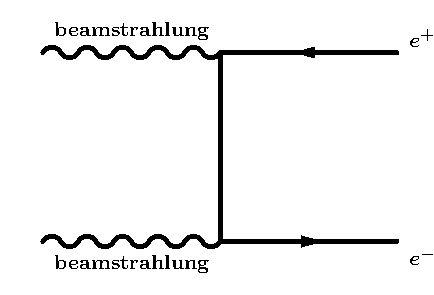
\includegraphics[width=0.48\textwidth]{figures/Breit-Wheeler.pdf}\\
 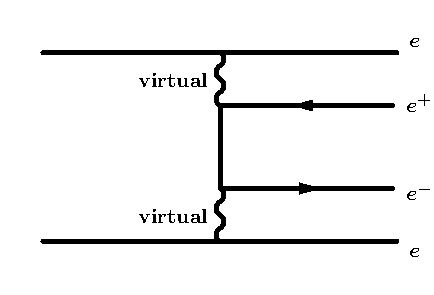
\includegraphics[width=0.48\textwidth]{figures/Landau-Lifshitz.pdf}
 \vspace*{0.5cm}
 \includegraphics[width=0.8\textwidth]{BeamDump_figures/Energy_deposition_xz_Design2.pdf}
 \end{column}
\end{columns}
\end{frame}

\subsection{Pair background study for the ILC250 stage}

\subsubsection{Pair background densities}
\begin{frame}{Pair background density in a 5\,T solenoid field}
The \alert{pair background particles spiral in the magnetic field}, and have a characteristic envelope.\\
In the new beam parameter sets, the \alert{beam emittance is reduced}. $\rightarrow$ Stronger beam-beam interactions, \alert{more background}!\\
The broader the envelope, the more particles reach the inner most layers of the detector.\\
\hspace*{1cm} ILC250 (Baseline design) \hfill New ILC250 set (reduced emittance)\hspace*{1cm}\\
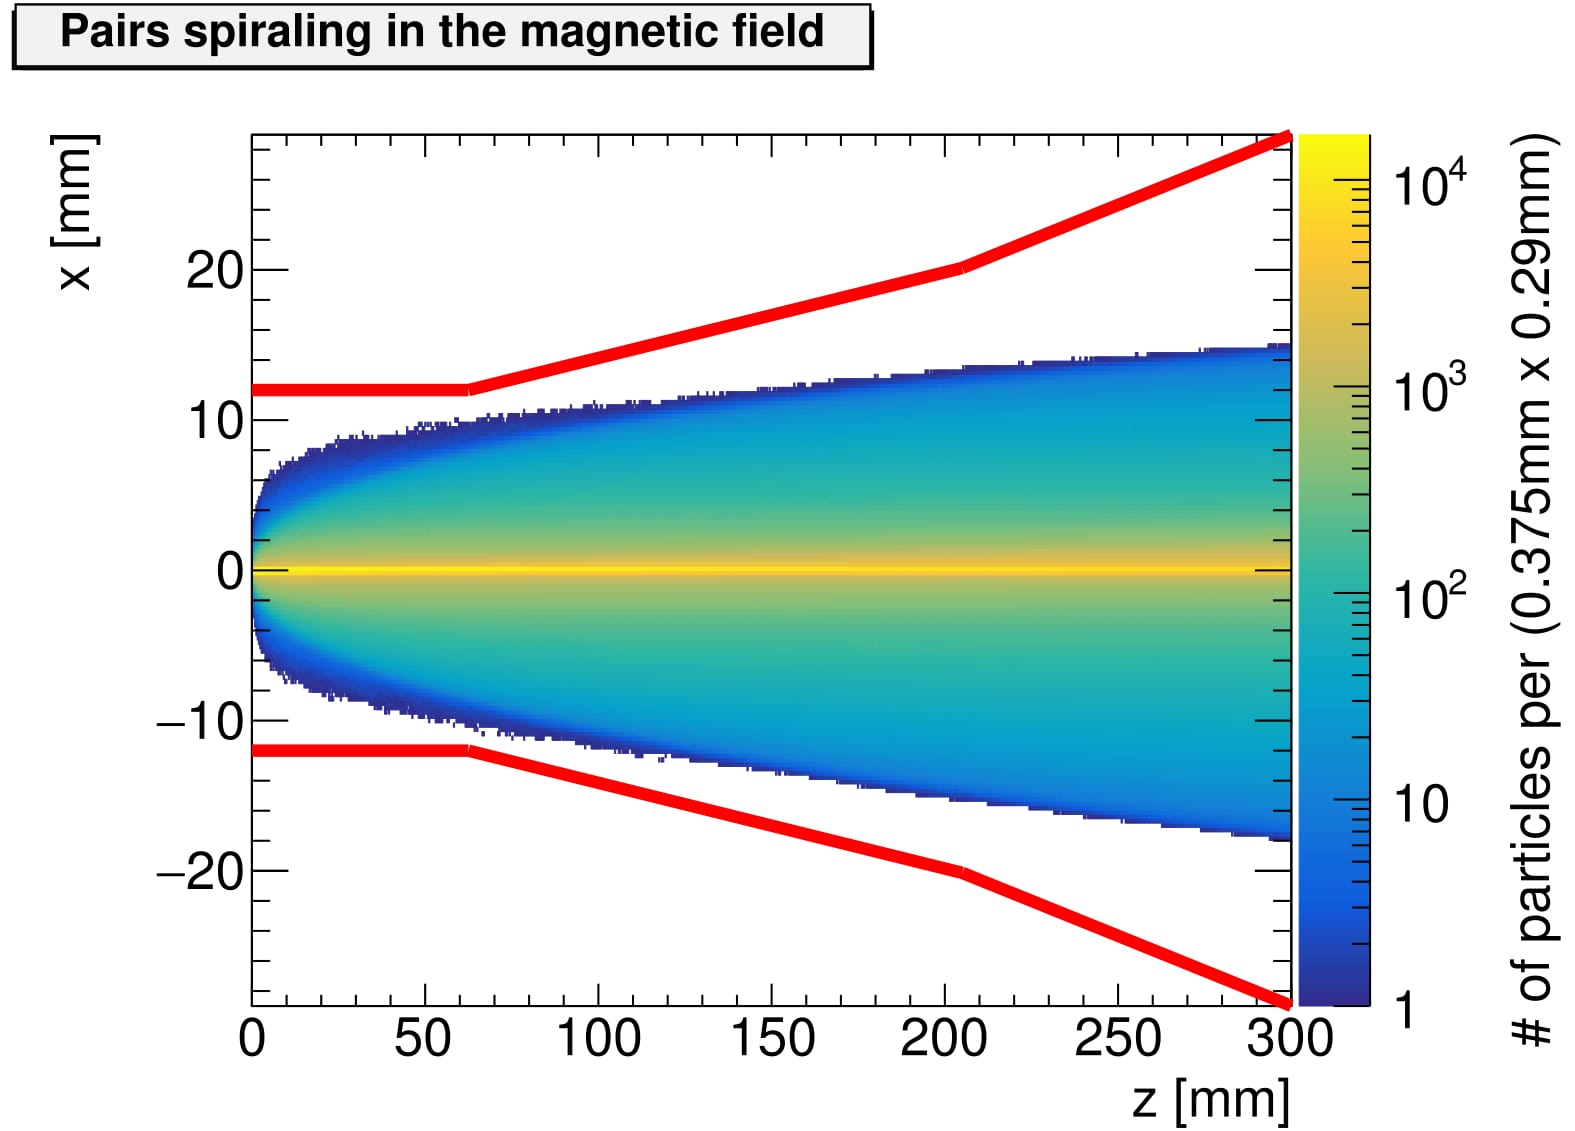
\includegraphics[width=0.49\textwidth]{ILC250_figures/Helix_tracks_xz_100bunches_250GeV_5T_DanielJeans-1.jpg}
\hspace*{0.1cm}
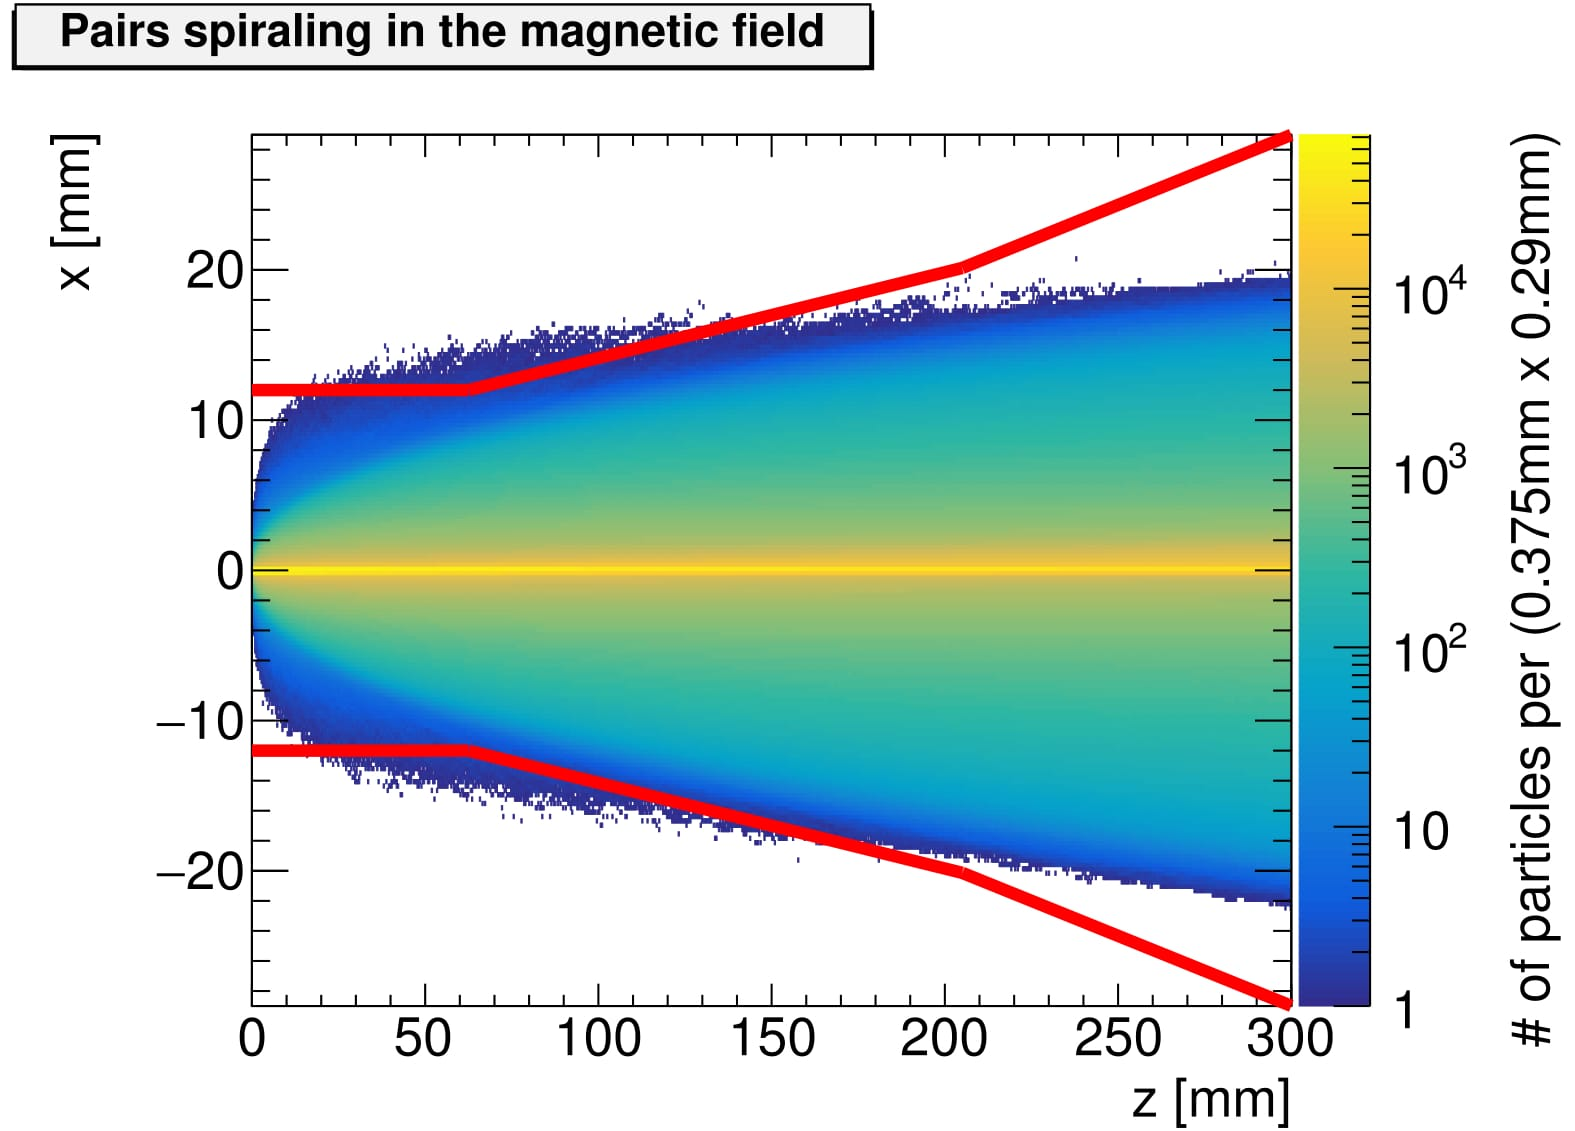
\includegraphics[width=0.49\textwidth]{ILC250_figures/Helix_tracks_xz_50bunches_250GeV_5T_Reduced_Emittance_x_Reduced_Beta_x-1.jpg}
\end{frame}

\subsubsection{SiD Occupancy}
\begin{frame}{SiD Vertex Detector Occupancy}
 Normalized Detector Occupancy: Number of cells containing a certain amount of hits, normalized by the total number of cells of the vertex detector.
\begin{center}
 Innermost layer of the Vertex Detector\\
 \includegraphics[width=0.55\textwidth]{ILC250_figures/Occupancy_Comparison_Layer_0_numcells_ILC250_ALL_SETS_6Sep2017_NEWSETNAMES.png}
\end{center}
SiD is confident that the occupancy can be accommodated in the design of the pixel detector.
\end{frame}

\subsection{The ILC Main Beam Dumps}
\subsubsection{Project Overview}
{
\usebackgroundtemplate{
\vbox to \paperheight{\vfil
 \tikz\node[opacity=0.1]{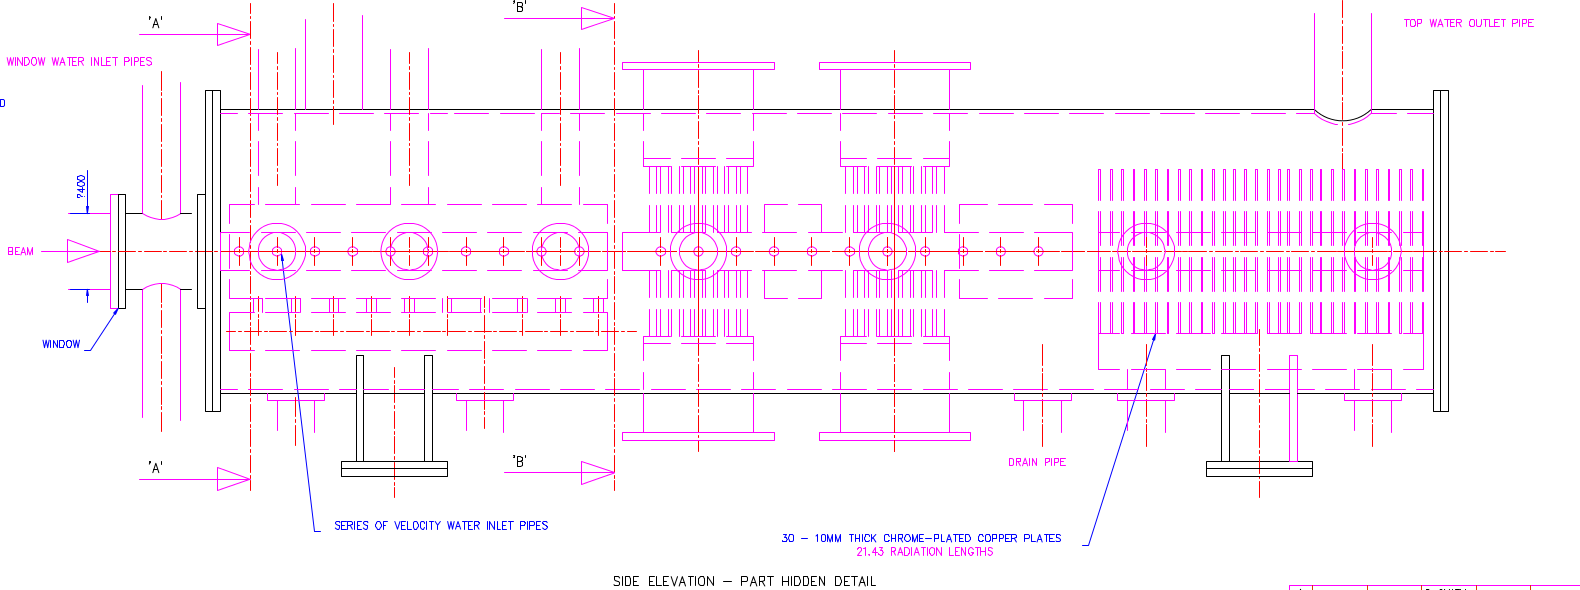
\includegraphics[width=\paperwidth]{BeamDump_figures/TB-0067-300-00-A_yz_view.png}};
 \vfil}
}
\begin{frame}{Neutron Background and Beam Dump Irradiation}
\flukalogo
The \alert{17\,MW}\footnote{13.7\,MW average beam power + 20\% margin} \alert{beam is dumped into a water tank} after collision.\\The activation of the dump surrounding will permit access to the dump area. Neutrons ($\lesssim$\SI{e10}{\per\square\centi\metre\per\year}) are emitted that irradiate the surroundings, and travel back towards the detectors.~\cite{SLAC_FLUKA}\\
\vspace*{0.1cm}
\alert{Goal: Simulating the energy deposition, irradiation, and background particles}
\begin{center}
  \hspace*{0.5cm} Water Beam Dump Design 1 \hfill Water Beam Dump Design 2 \hspace*{0.5cm} \\
  \includegraphics[width=0.5\textwidth]{BeamDump_figures/Design1_geometry.png}
  \hspace*{0.1cm}
  \includegraphics[width=0.5\textwidth]{BeamDump_figures/Design2_geometry.png}
\end{center}
\end{frame}
}

\subsubsection{The FLUKA simulation}
\begin{frame}{Deposited Energy per bunch}
\begin{center}
\hspace*{1.6cm} Design 1 \hfill Design 2 \hspace*{1.8cm} \\
  \includegraphics[width=0.52\textwidth]{BeamDump_figures/Energy_deposition_xz_Design1.pdf}
    \includegraphics[width=0.52\textwidth]{BeamDump_figures/Energy_deposition_xz_Design2.pdf}
\end{center}
 Shielding walls seem to stop particles fluxes well, but large scattering in Design 2 at high water pressure sections leads to energy deposition outside the walls.
\end{frame}

\begin{frame}
\textbf{After one month of beam operation}, the beam is turned off.\\
  \begin{center}
    \hspace*{1.4cm} Instantaneous \hfill After 1 year\hspace*{2cm} \\
  \includegraphics[width=0.5\textwidth]{BeamDump_figures/Dose_equivalent_total_Design1.pdf}
  \includegraphics[width=0.5\textwidth]{DoseEQ_Time/Design1_5.pdf}
 \end{center}
\end{frame}
\begin{frame}{Dose Rate over Time}
The dose rate measured at the longitudinal shower maximum inside the vessel over time:
\begin{center}
  \includegraphics[width=0.7\textwidth]{BeamDump_figures/DoseEQ_Time_Comparison.pdf}
\end{center}
\textbf{After one year}, the dose rate drops to \\\textbf{$\sim$ 0.1\,mSv/s} for \textcolor{Red}{Design 1} and to \textbf{$\sim$ 10\,mSv/s} for \textcolor{Blue}{Design 2}.
\end{frame}

\section{Summary and Outlook}
\begin{frame}
Understanding the backgrounds occurring at a collider is crucial for the design of both, the machine and the detectors.
\vspace*{0.2cm}
 \begin{itemize} 
  \item Studying the \textbf{pair background} wrt timing, origin and envelopes for 500, 350 and 250\,GeV ILC staging scenarios is \alert{essential for the design of the beam pipe, the vertex detector and the sensors}
  \item Simulating the \textbf{Main Beam Dump} and the EXT line with FLUKA is \alert{crucial for understanding the irradiation of the dump surrounding and the detector neutron background}
  \item More backgrounds studies have been done...
 \end{itemize}
\vspace*{0.5cm}
\alert{All simulation studies are important for the last steps towards the ILC!}
\end{frame}


\section*{The end}
{
\usebackgroundtemplate{
 \tikz\node[opacity=0.1]{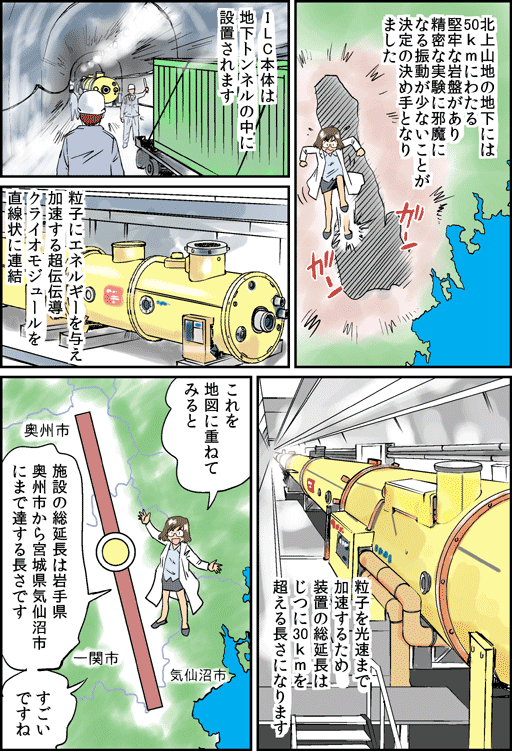
\includegraphics[width=\paperwidth,resolution=200]{figures/ilc-Comic.png}};
 % \tikz\node[opacity=0.2]{\centering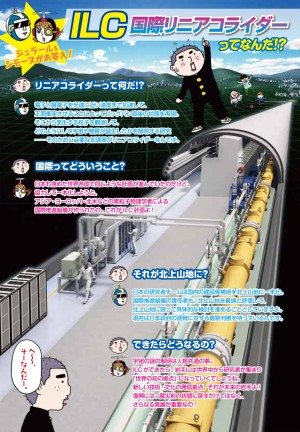
\includegraphics[height=\paperheight]{figures/Iwatecomics.jpg}};
 }
\begin{frame}
\ilclogo
\begin{center}
If you are interested in SiD and keen on working for the ILC, \\
if you like working in a very international environment, \\
or if you love Japan,\\
there are lots of possible Master's and Ph.D topics.\\
\vspace*{1cm}
\textcolor{RubineRed}{
	\LARGE Thanks!
	%\\
	%\begin{CJK}{UTF8}{min}
	%どうもありがとうございます。
	%\end{CJK}
}
\end{center}
\end{frame}
}

\section*{References}
\begin{thebibliography}{9}
\begin{frame}{References}
\bibitem{TDR} T. Behnke, et al.
\emph{The International Linear Collider - Technical Design Report}, 2013.
\bibitem{LHC TDR} \emph{LHC - Design Report}, \url{http://ab-div.web.cern.ch/ab-div/Publications/LHC-DesignReport.html}
\bibitem{IP beam parameters} ATLAS-CONF-2010-027. \emph{Characterization of Interaction-Point Beam Parameters Using the pp Event-Vertex Distribution Reconstructed in the ATLAS Detector at the LHC}, 2010. \url{http://cds.cern.ch/record/1277659/files/ATLAS-CONF-2010-027.pdf}
\bibitem{ILCPAC2012} M. Peskin. \emph{Physics Motivation for the ILC}, 2012. \url{http://www.fnal.gov/directorate/ILCPAC/2012Dec/Physics-ILCPAC2012-Peskin.pdf}
\end{frame}
\begin{frame}{References}
\bibitem{MIT2013} Klute, Markus, Rémi Lafaye, Tilman Plehn, Michael Rauch, and
Dirk Zerwas. \emph{Measuring Higgs Couplings at a Linear Collider}
EPL (Europhysics Letters) 101, no. 5 (March 1, 2013): 51001. \url{http://dx.doi.org/10.1209/0295-5075/101/51001}
\bibitem{RHUL} Mark Thomson. \emph{Physics and Detectors at the ILC}, 2013. \url{https://www.royalholloway.ac.uk/physics/documents/pdf/events/particlephysicsseminars/13-14markthomson23oct2013.pdf}
\bibitem{ATF2} Kuroda et al. \emph{A plan of KEK-ATF Final Focus Test Beam Line (ATF2)
}. \url{http://icfa-nanobeam.web.cern.ch/icfa-nanobeam/paper/urakawa_ATF2-2.pdf}

\end{frame}
\end{thebibliography}

%--------------------------------------------------------------------------------
\appendix

\begin{frame}
\begin{center}
\LARGE Additional Material
\end{center}
  \tableofcontents
\end{frame}

\section{ILC}
\subsection{ILC parameters}
\begin{frame}{ILC baseline parameters}
\ilclogo
\centering
	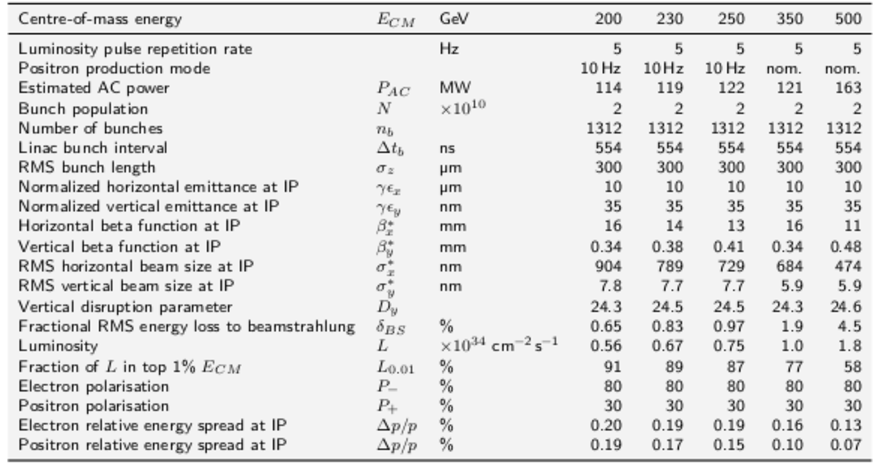
\includegraphics[width=\textwidth]{figures/ILCTDR-VOLUME_3-PART_II_ILCparameters.pdf}
\end{frame}
\begin{frame}{ILC parameters for the different upgrade stages}
\ilclogo
\centering
	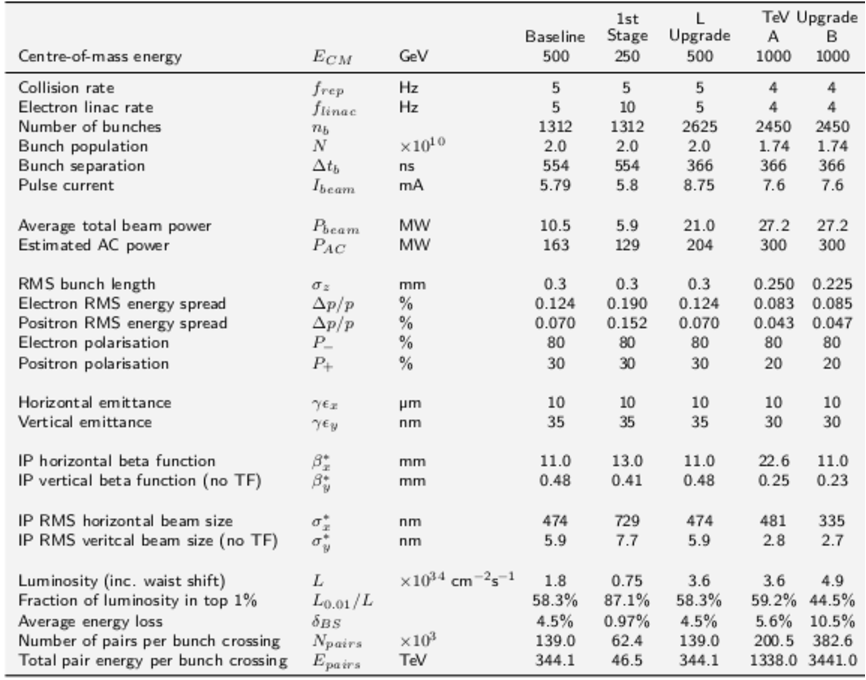
\includegraphics[width=0.8\textwidth]{figures/ILCTDR-VOLUME_3-PART_II_ILCparametersUpgrades.pdf}
\end{frame}

\subsection{Basic accelerating structure}
\begin{frame}{Basic accelerating structure}
\ilclogo
The main accelerating structures are the two 11km long LINACs.
\begin{itemize}
\item 9-cell superconducting RF cavities operating at 1.3 GHz 
\item Accelerating gradient of >30 MV/m
\item Electrons and positrons accelerated in RF standing waves in the cavities 
\end{itemize}
\begin{center}
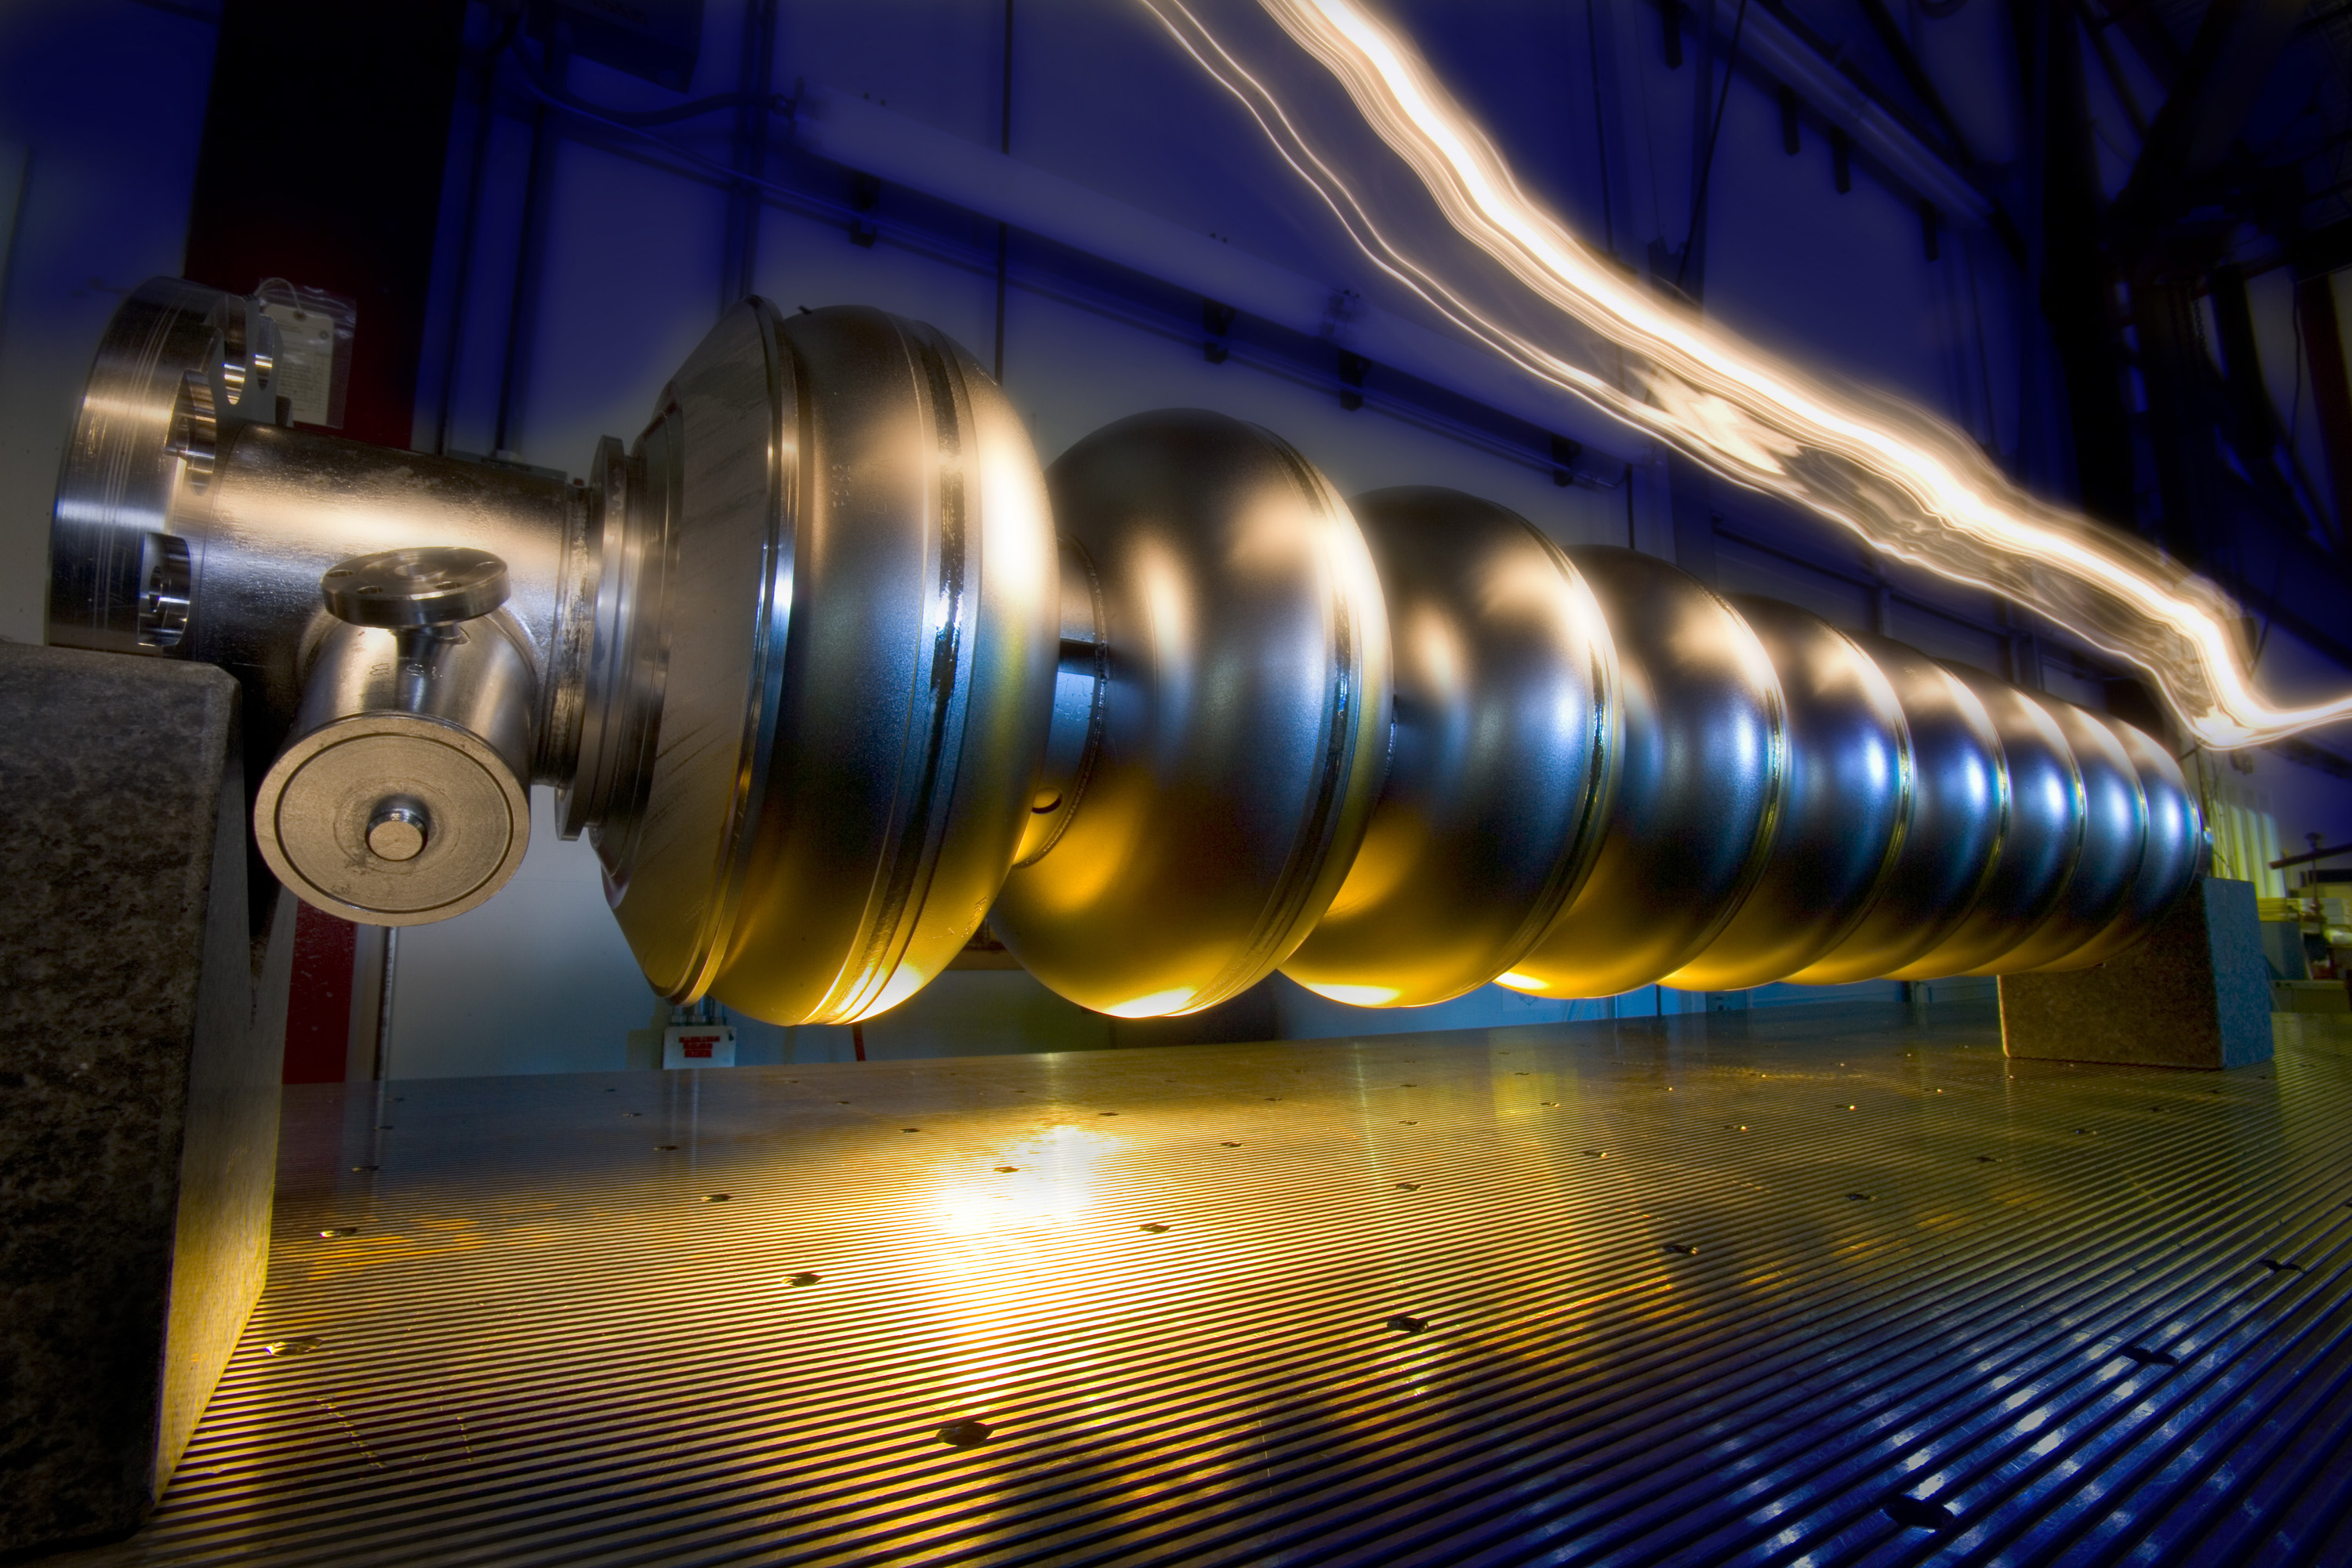
\includegraphics[width=0.45\textwidth]{figures/cavity.jpg}
\end{center}
The cavities are also developed, built and tested at DESY.
\end{frame}

\subsection{The Final-Focus system}
\begin{frame}{The Final-Focus system}
 \ilclogo
 The Final-Focus (FF) uses:
\begin{itemize}
 \item Strong compact superconducting quadrupoles to focus the
beam at the IP (single collision point with a 14 mrad beam-crossing angle)
\item Sextupoles providing local chromaticity correction
\item Two superconducting octupole doublets, which use nonlinear
focusing to reduce the amplitude of beam-halo particles while leaving the beam core untouched $\rightarrow$ permitting larger collimation amplitude
\item Collimators and spoilers to prevent the beam halo and background particles from entering the detectors
\end{itemize}
\end{frame}

\section{Pair background}
\subsection{New beam parameter sets for the ILC250}
\begin{frame}{The beam parameters of the \textbf{ILC250}}
\ilclogo
\alert{Going from ILC500 to ILC250}: New beam parameters under discussion in order to increase the luminosity:
\begin{table}[]
\centering
\begin{tabularx}{\textwidth}{ll|rrrr}
\hline
& & \multicolumn{1}{>{\centering}p{1.5cm}}{\textbf{TDR Baseline}} & \textbf{Set (A)} & \textbf{Set (B)} & \textbf{Set (C)}\\ 
\hline
\cline{1-6}
\hline
E$_{CM}$  &[\si{\GeV}] & 250  & 250  & 250 & 250\\
n$_b$ & & \num{1312} & \num{1312} & \num{1312} &  \num{1312} \\
N & & \num{2.0e10}  & \num{2.0e10}  & \num{2.0e10}  & \num{2.0e10}\\
$\epsilon_x^*$ &[\si{\micro\metre}] & 10  & \textbf{5}  &  \textbf{5} & \textbf{5}\\
$\epsilon_y^*$ &[\si{\nano\metre}] & 35 &  35  &  35 & 35\\
$\beta_x^*$ &[\si{\milli\metre}] & 13  &  13  &  \textbf{9.19} & \textbf{9.19}\\
$\beta_y^*$ &[\si{\milli\metre}] & 0.41  &  0.41  &  0.41 & \textbf{0.58}\\
\lumi &[\si{\per\centi\metre\squared\per\second}] & \num{0.8e34} & \num{1.37e34} & \num{1.97e34} & \num{1.80e34}\\
\hline
\end{tabularx}
\end{table}
\begin{flushright}
 \small Work in progress... 
\end{flushright}
\alert{Reduced emittance leads to stronger beam-beam interactions, and therefore to increased \positron \electron pair background.}
\end{frame}

\subsection{Pair background helixes}
\begin{frame}{Pair background -  P\textsubscript{T}}
\sidlogo
Since their P\textsubscript{T} ranges between 0 and 2\,GeV, they form \textbf{helix tracks in the solenoid field}. The tracks extend to the inner detector layers, and leave up to several tens of hits.
\begin{center}
\includegraphics[width=0.7\textwidth]{figures/PT_hittime_primaries_SiVertexEndcapSiVertexBarrel.pdf}
\end{center}
\end{frame}

\begin{frame}{Explanation of helix track calculations}
 \begin{center}
  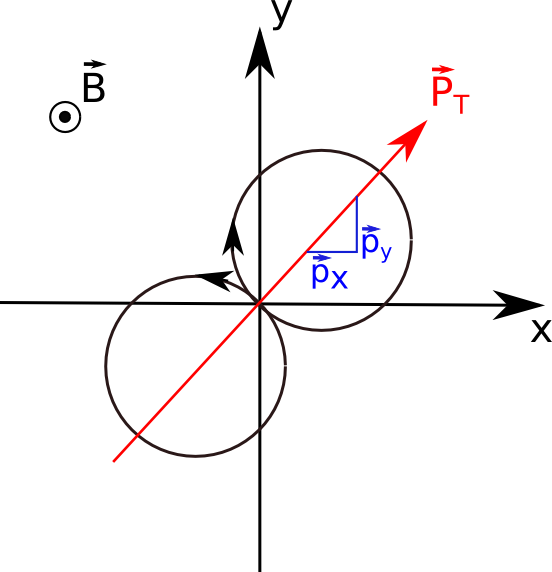
\includegraphics[width=0.65\textwidth]{figures/Helix_explanation.png}
\end{center}
\end{frame}

\subsubsection{Pair background densities}
\begin{frame}{Pair background density in a 5\,T solenoid field}
 \begin{figure}
\centering
\begin{subfigure}[t]{0.35\textwidth}
\centering
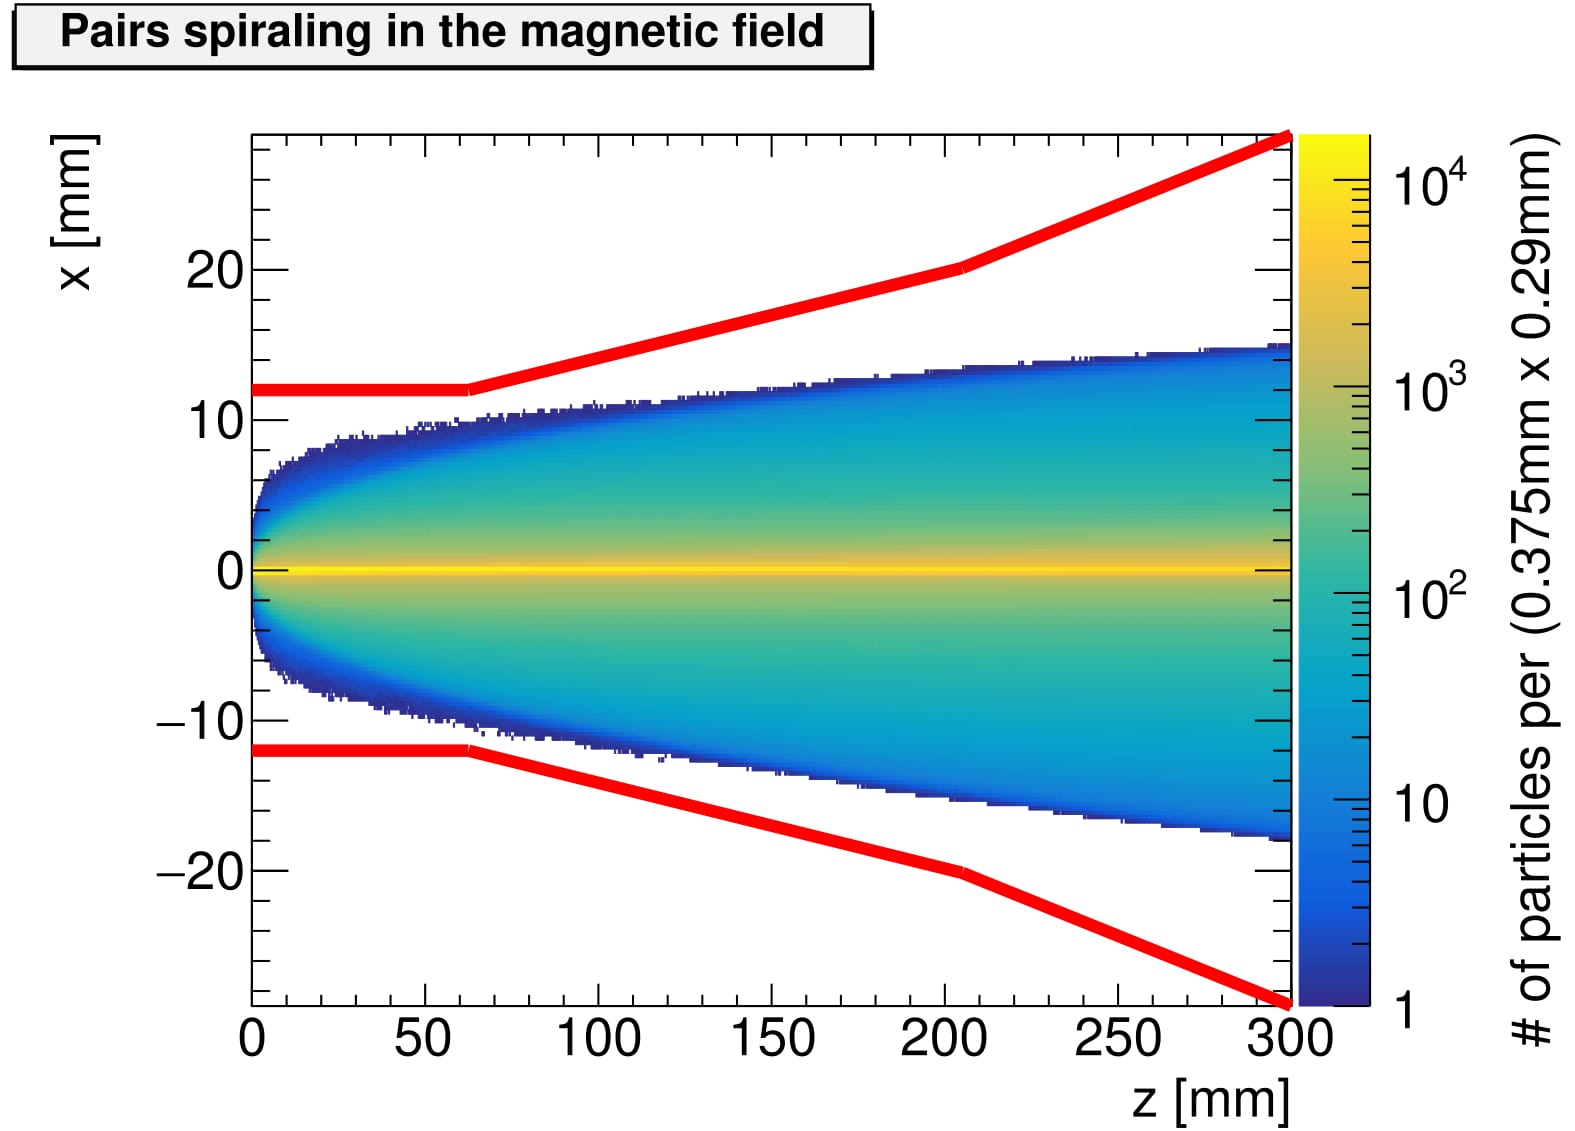
\includegraphics[width=\textwidth]{ILC250_figures/Helix_tracks_xz_100bunches_250GeV_5T_DanielJeans-1.jpg}
\caption{ILC250 set (TDR)}
\end{subfigure}
\hspace*{0.1cm}
\begin{subfigure}[t]{0.35\textwidth}
\centering
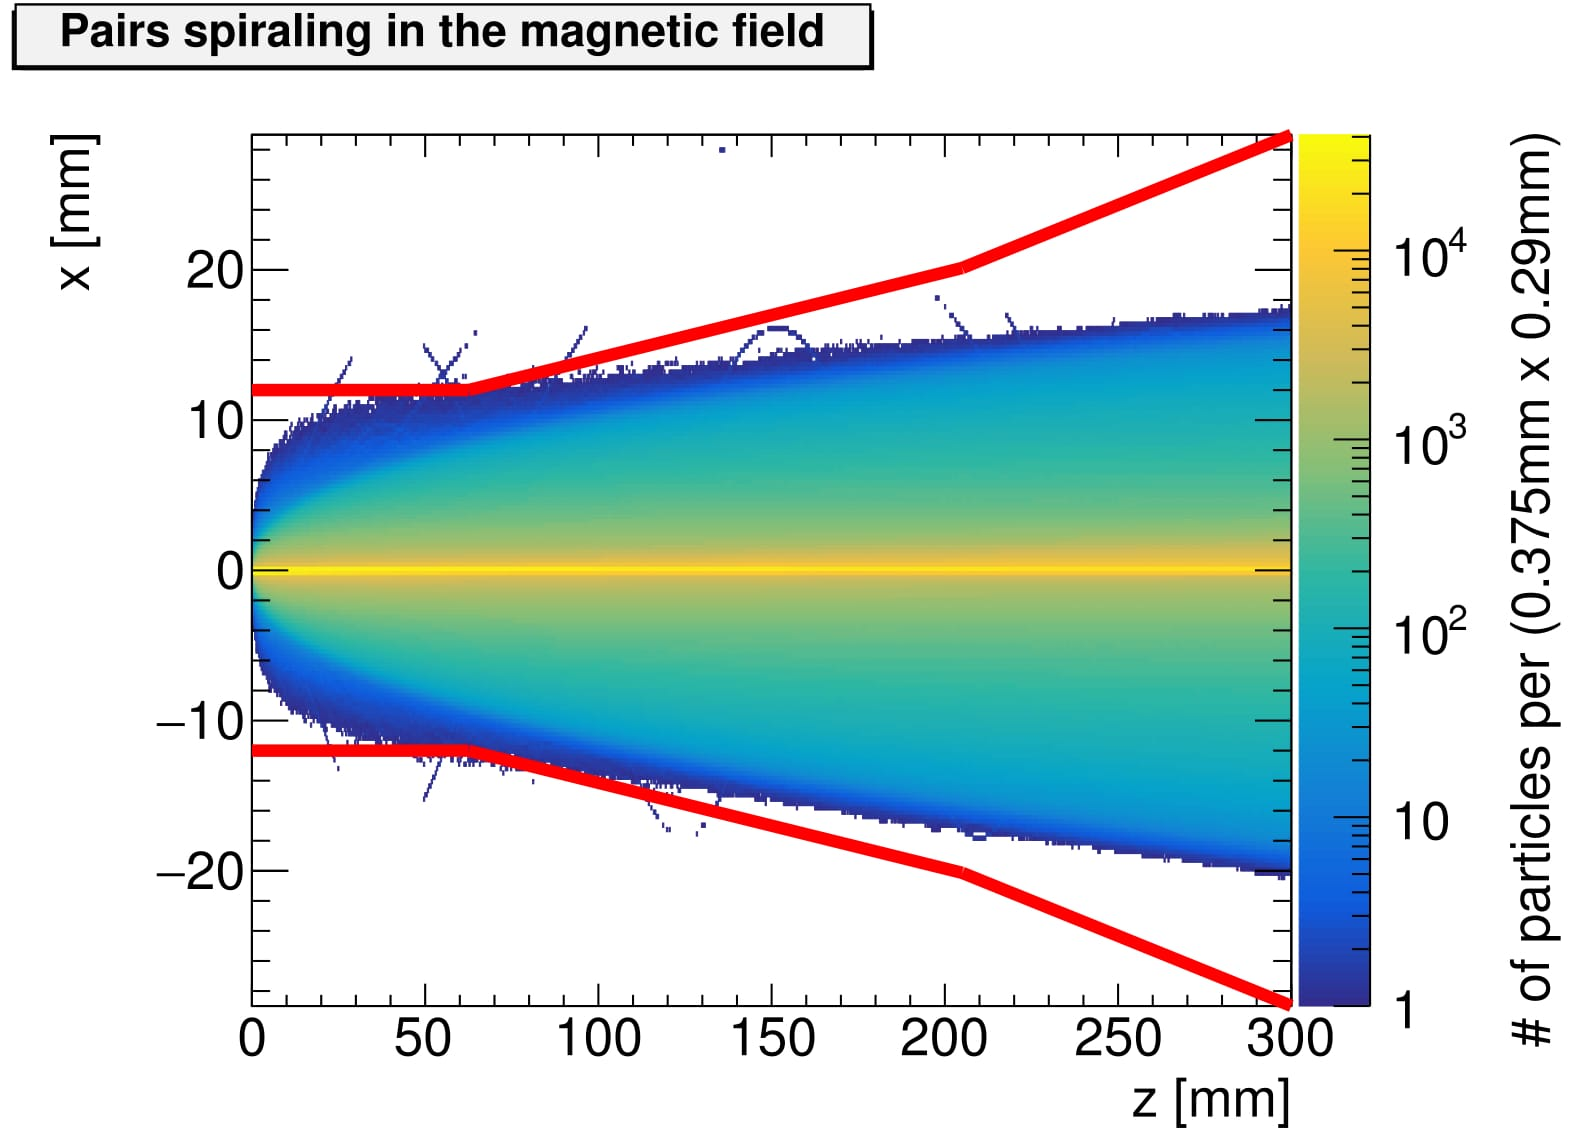
\includegraphics[width=\textwidth]{ILC250_figures/Helix_tracks_xz_80bunches_250GeV_5T_Reduced_Emittance_x-1.jpg}
\caption{ILC250 set (A)}
\end{subfigure}
\\
\begin{subfigure}[t]{0.35\textwidth}
\centering
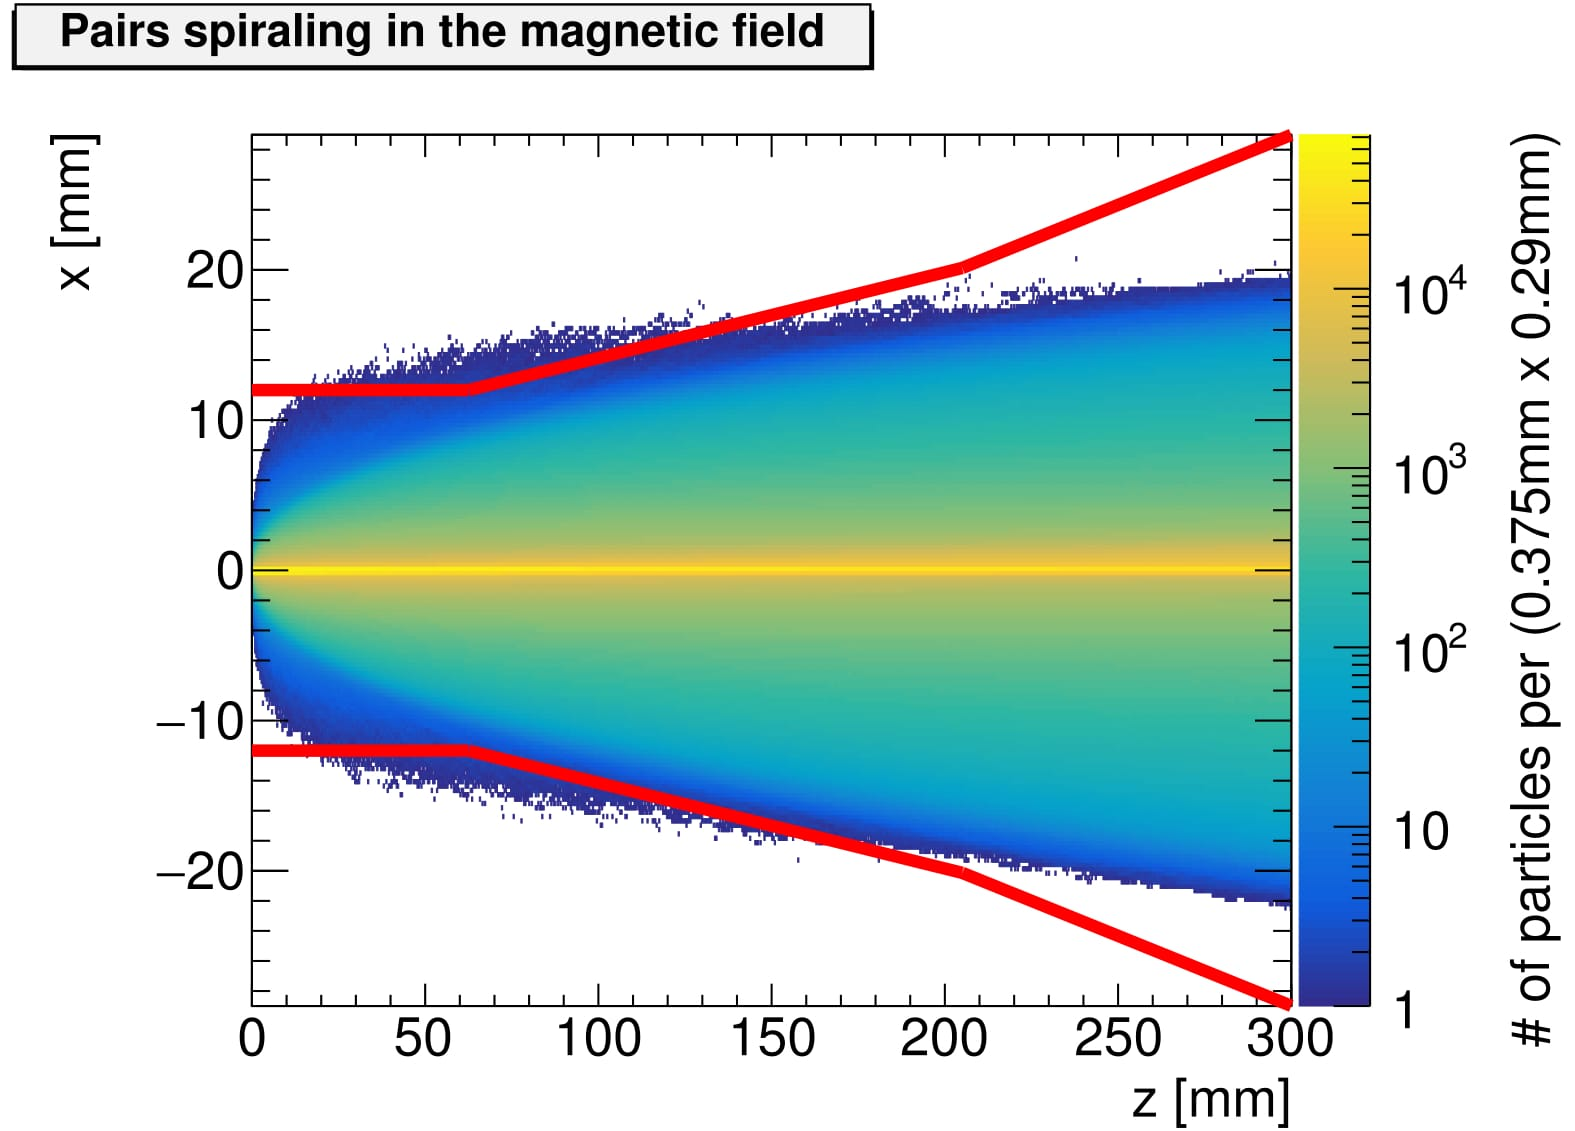
\includegraphics[width=\textwidth]{ILC250_figures/Helix_tracks_xz_50bunches_250GeV_5T_Reduced_Emittance_x_Reduced_Beta_x-1.jpg}
\caption{ILC250 set (B)}
\end{subfigure}
\hspace*{0.1cm}
\begin{subfigure}[t]{0.35\textwidth}
\centering
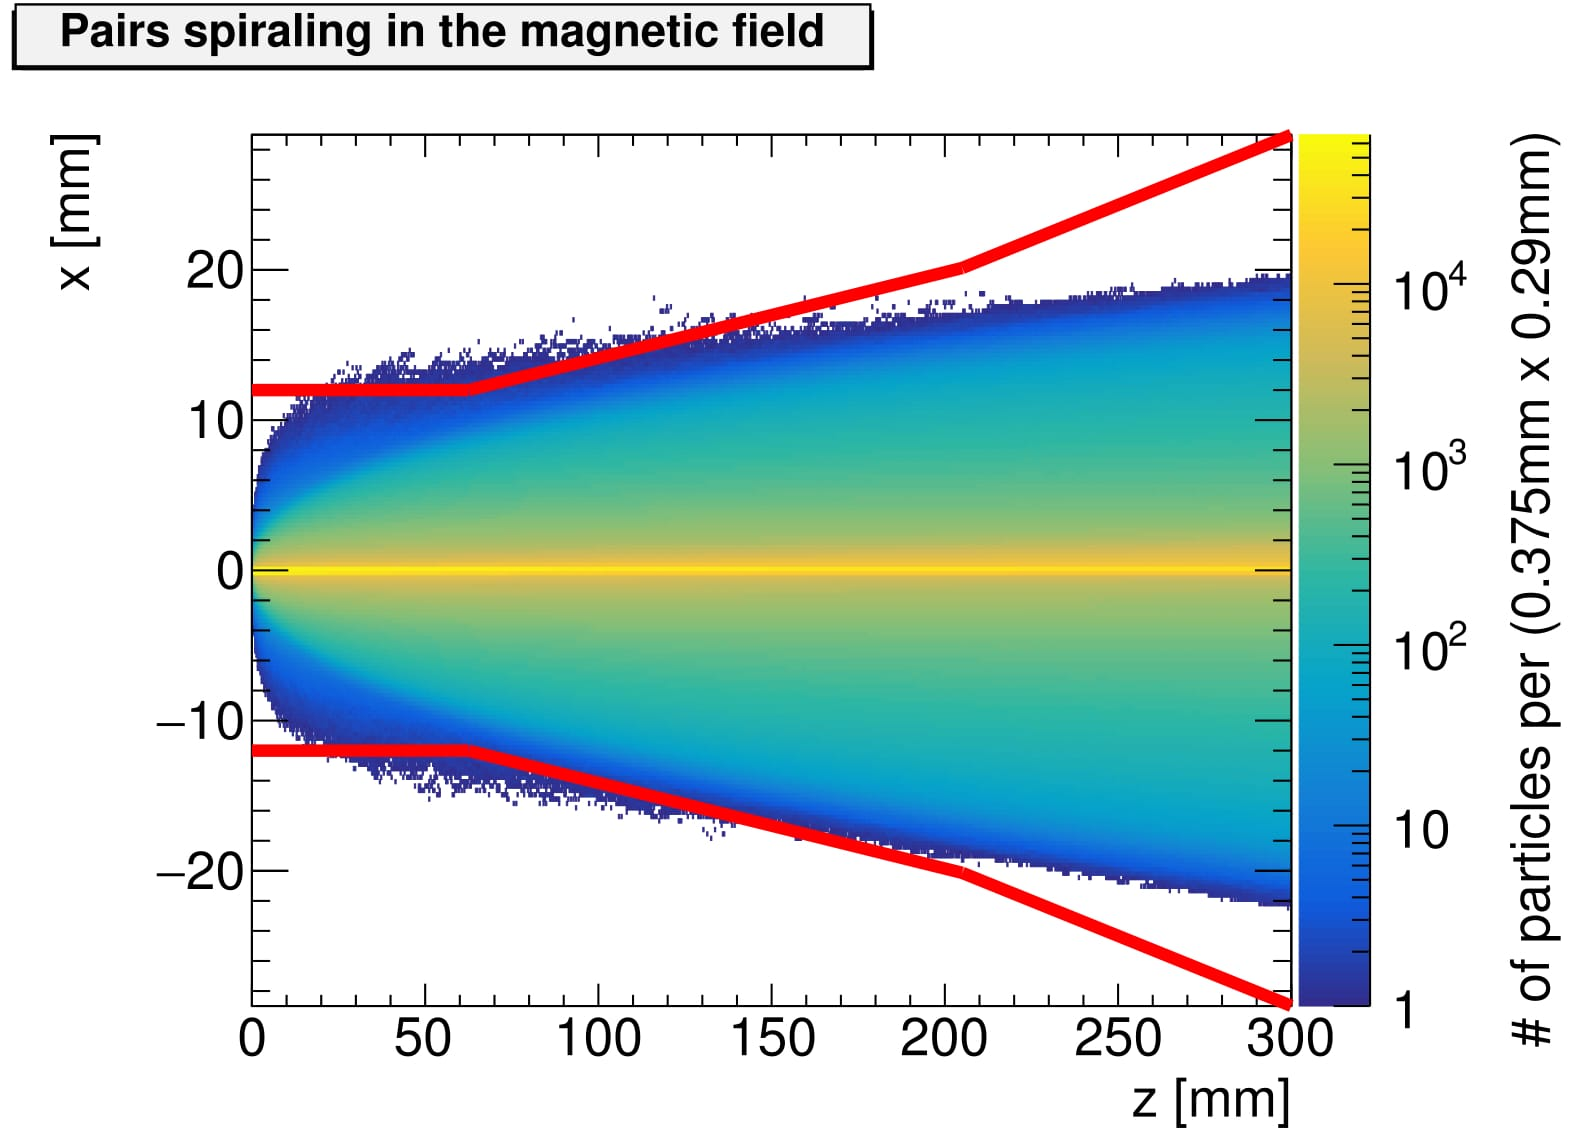
\includegraphics[width=\textwidth]{ILC250_figures/Helix_tracks_xz_50bunches_250GeV_5T_Reduced_Emittance_x_Reduced_Beta_x_Increased_Beta_y-1.jpg}
\caption{ILC250 set (C)}
\end{subfigure}
\caption{Pair background density for the different ILC250 beam parameter sets.
The beam pipe is represented by the red solid lines.}
\label{fig:Envelopes}
\end{figure}

\end{frame}

\begin{frame}{Projection of the pair background density along x}
\begin{center}
 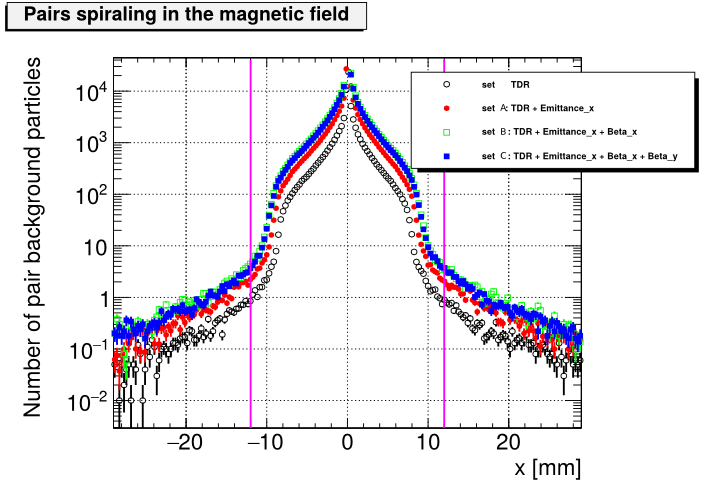
\includegraphics[width=0.72\textwidth]{ILC250_figures/HelixEnvelope_Projection_Comparison_250GeV_parametersets_NEWSETNAMES.png}
\end{center}
The envelopes are in all schemes well contained within the beam pipe. Less than 10 particles per bunch crossing are to be expected outside the beam pipe.
\end{frame}

\subsection{SiD Occupancy}
\begin{frame}{SiD Vertex Detector Occupancy}
 Normalized Detector Occupancy: Number of cells containing a certain amount of hits, normalized by the total number of cells of the vertex detector.
 \begin{figure}
\centering
\begin{subfigure}[t]{0.48\textwidth}
\centering
\includegraphics[width=\textwidth]{ILC250_figures/Occupancy_Comparison_All_layers_wrt__cells_ILC250_ALL_SETS_6Sep2017_NEWSETNAMES.png}
\caption{\alert{Normalized Occupancy for all layers}}
\end{subfigure}
\hspace*{0.2cm}
\begin{subfigure}[t]{0.48\textwidth}
\centering
\includegraphics[width=\textwidth]{ILC250_figures/Occupancy_Comparison_Layer_0_numcells_ILC250_ALL_SETS_6Sep2017_NEWSETNAMES.png}
\caption{\alert{Normalized Occupancy for layer 0}}
\end{subfigure}
\end{figure}
SiD is confident that the occupancy can be accommodated in the design of the pixel detector.
\end{frame}

\end{document}
